% i still have no clue how i wanna do this
% doing everything for all texts and 1, 2, 4, 8 and 16 threads is way too much
% maybe i can reduce the set of texts to just "interesting" ones
% maybe i can also discard some of my implementations that are not on the pareto front

\documentclass[a4]{article}

\usepackage[utf8]{inputenc}
\usepackage[english]{babel}

\usepackage{amsmath,amsfonts,amssymb}
\usepackage{fullpage}
\usepackage{verbatim}

\usepackage{tikz,pgfplots}
\usetikzlibrary{patterns, patterns.meta}
\usepgfplotslibrary{groupplots}



\pgfplotscreateplotcyclelist{wtddcycles} {
  red, every mark/.append style = {solid}, mark = square*\\
  black, every mark/.append style = {solid}, mark = square*\\
  orange!75!black, every mark/.append style = {solid}, mark = square*\\
  blue, every mark/.append style = {solid}, mark = triangle*\\
  green!50!black, every mark/.append style = {solid}, mark = triangle*\\
  violet, every mark/.append style = {solid}, mark = triangle*\\  
}


\pgfplotsset{
    major grid style = { thin, dotted, color = black!50 },
    minor grid style = { thin, dotted, color = black!50 },
    grid,
    ymin = 0,
    legend cell align = left,
    legend pos = north west,
	  /pgfplots/ybar legend/.style = {
		  /pgfplots/legend image code/.code={%
			  \draw[##1,/tikz/.cd,yshift=-0.35em]
      (0cm,0cm) rectangle (0.7em,0.8em);},
	  },  
}


\begin{document}

\title{WT Benchmark}
\author{Jan-Philipp Tarnowski}
\maketitle

\clearpage


% IMPORT-DATA stats ../results-pcc-regular.out

% IMPORT-DATA stats_a ../results-lightweight-regular.out
% IMPORT-DATA stats_b ../results-large.out
% IMPORT-DATA stats_c ../results-pcc-dd.out
% IMPORT-DATA stats_d ../results-lightweight-dd.out
% IMPORT-DATA stats_e ../results-dd-large.out

% TODO - large dd texts

% SQL INSERT INTO stats SELECT * FROM stats_a
% SQL INSERT INTO stats SELECT * FROM stats_b
% SQL INSERT INTO stats SELECT * FROM stats_c
% SQL INSERT INTO stats SELECT * FROM stats_d
% SQL INSERT INTO stats SELECT * FROM stats_e

% Normalize DS Names and orders
% SQL UPDATE stats SET type = 'lwtlut1644', ds_order = 0 WHERE type LIKE 'lwt%lut_16_4_4%'
% SQL UPDATE stats SET type = 'lwtpext164', ds_order = 1 WHERE type LIKE 'lwt%pext_16_4%'
% SQL UPDATE stats SET type = 'lwtshuffle648', ds_order = 2 WHERE type LIKE 'lwt%shuffle_64_8%'
% SQL UPDATE stats SET type = 'lwtpwmpc', ds_order = 3 WHERE type LIKE 'pwm_%_pcI%tree'
% SQL UPDATE stats SET type = 'lwtpwmpcss', ds_order = 4 WHERE type LIKE 'pwm_%_pc_ssI%tree'
% SQL UPDATE stats SET type = 'lwtpwmps', ds_order = 5 WHERE type LIKE 'pwm_%_psI%tree'

% SQL UPDATE stats SET type = 'wmlut1644', ds_order = 0 WHERE type LIKE 'wm%lut_16_4_4%'
% SQL UPDATE stats SET type = 'wmpext88', ds_order = 1 WHERE type LIKE 'wm%pext_8_8%'
% SQL UPDATE stats SET type = 'wmshuffle648', ds_order = 2 WHERE type LIKE 'wm%shuffle_64_8%'
% SQL UPDATE stats SET type = 'wmpwmpc', ds_order = 3 WHERE type LIKE 'pwm_%_pcI%matrix'
% SQL UPDATE stats SET type = 'wmpwmpcss', ds_order = 4 WHERE type LIKE 'pwm_%_pc_ssI%matrix'
% SQL UPDATE stats SET type = 'wmpwmps', ds_order = 5 WHERE type LIKE 'pwm_%_psI%matrix'

% SQL UPDATE stats SET ext_split = time_in_s WHERE threads = 1

% SQL DELETE FROM stats WHERE type LIKE '%\_%' ESCAPE '\'


% SQL UPDATE stats SET file = 'dblp.xml' WHERE file LIKE '%/dblp.xml'
% SQL UPDATE stats SET file = 'dna' WHERE file LIKE '%/dna'
% SQL UPDATE stats SET file = 'english' WHERE file LIKE '%/english'
% SQL UPDATE stats SET file = 'pitches' WHERE file LIKE '%/pitches'
% SQL UPDATE stats SET file = 'proteins' WHERE file LIKE '%/proteins'
% SQL UPDATE stats SET file = 'sources' WHERE file LIKE '%/sources'

% SQL UPDATE stats SET file = 'chr22.dna' WHERE file LIKE '%/chr22.dna'
% SQL UPDATE stats SET file = 'etext99' WHERE file LIKE '%/etext99'
% SQL UPDATE stats SET file = 'gcc-3.0.tar' WHERE file LIKE '%/gcc-3.0.tar'
% SQL UPDATE stats SET file = 'howto' WHERE file LIKE '%/howto'
% SQL UPDATE stats SET file = 'jdk13c' WHERE file LIKE '%/jdk13c'
% SQL UPDATE stats SET file = 'linux-2.4.5.tar' WHERE file LIKE '%/linux-2.4.5.tar'
% SQL UPDATE stats SET file = 'rctail96' WHERE file LIKE '%/rctail96'
% SQL UPDATE stats SET file = 'rfc' WHERE file LIKE '%/rfc'
% SQL UPDATE stats SET file = 'sprot34.dat' WHERE file LIKE '%/sprot34.dat'
% SQL UPDATE stats SET file = 'w3c2' WHERE file LIKE '%/w3c2'

% SQL UPDATE stats SET file = 'cc.16gib' WHERE file LIKE '%/cc.txt'
% SQL UPDATE stats SET file = 'dna.16gib' WHERE file LIKE '%/dna.txt'
% SQL UPDATE stats SET file = 'wiki.16gib' WHERE file LIKE '%/wiki.txt'




\clearpage

\begin{figure}[t]
\begin{center}
    \begin{tikzpicture}
        \begin{groupplot} [
            width = 0.4\textwidth,
            height = 6.4cm,
            enlarge x limits = 0.075,
            group style = { 
                vertical sep = 1.0cm,
                horizontal sep = 0.0cm,
                group size = { 
                    3 by 3
                } 
            },
            cycle list name = wtddcycles,
            legend style = { 
                at = {(0.5, -0.275)},
                anchor = north,
                legend columns = 6,
                column sep = 2ex
            },
            ylabel style = {
                at = {(0.11, 0.5)}
            },
            title style = {
                at = {(0.5, 0.96)}
            },
            xticklabels = { , 1, 2, 4, 8, 16 },
            xtick distance = 1,
            ytick distance = 1,
            ymax = 7.0,
        ]
        
        
        \nextgroupplot [
            title = dblp.xml,
            ylabel = $\text{GiBit} / s$,
        ]


			%% MULTIPLOT(type) SELECT LOG(2, threads) AS x, MEDIAN((alpha_bits * (size / CAST(time_in_s AS Float))) / (1024 * 1024 * 1024)) AS y,MULTIPLOT
			%% FROM stats WHERE (type LIKE 'lwt%') AND (file LIKE 'dblp.xml') GROUP BY MULTIPLOT,x ORDER BY ds_order,MULTIPLOT,x
   \addplot coordinates { (0.0,0.423277) (1.0,0.805035) (2.0,1.4801) (3.0,2.82811) (4.0,2.97692) };
   \addlegendentry{type=lwtlut1644};
   \addplot coordinates { (0.0,0.705278) (1.0,1.26055) (2.0,2.25815) (3.0,4.00846) (4.0,4.29409) };
   \addlegendentry{type=lwtpext164};
   \addplot coordinates { (0.0,1.44314) (1.0,2.17009) (2.0,3.14611) (3.0,4.06877) (4.0,3.98953) };
   \addlegendentry{type=lwtshuffle648};
   \addplot coordinates { (0.0,0.594173) (1.0,1.15243) (2.0,2.25656) (3.0,4.49742) (4.0,6.01785) };
   \addlegendentry{type=lwtpwmpc};
   \addplot coordinates { (0.0,0.734843) (1.0,1.41961) (2.0,2.80362) (3.0,5.44622) (4.0,5.82952) };
   \addlegendentry{type=lwtpwmpcss};
   \addplot coordinates { (0.0,0.570799) (1.0,1.10154) (2.0,2.16651) (3.0,4.28371) (4.0,5.3366) };
   \addlegendentry{type=lwtpwmps};


            \legend{};

   \nextgroupplot [
    ylabel = ,
    yticklabels = {},
    title = dna
]


    %% MULTIPLOT(type) SELECT LOG(2, threads) AS x, MEDIAN((alpha_bits * (size / CAST(time_in_s AS Float))) / (1024 * 1024 * 1024)) AS y,MULTIPLOT
    %% FROM stats WHERE (type LIKE 'lwt%') AND (file LIKE 'dna') GROUP BY MULTIPLOT,x ORDER BY ds_order,MULTIPLOT,x
    \addplot coordinates { (0.0,0.516911) (1.0,0.990253) (2.0,1.87017) (3.0,3.14996) (4.0,3.82189) };
    \addlegendentry{type=lwtlut1644};
    \addplot coordinates { (0.0,0.862305) (1.0,1.54148) (2.0,2.83026) (3.0,4.27393) (4.0,5.50718) };
    \addlegendentry{type=lwtpext164};
    \addplot coordinates { (0.0,0.987743) (1.0,1.87797) (2.0,2.9713) (3.0,3.73286) (4.0,4.11103) };
    \addlegendentry{type=lwtshuffle648};
    \addplot coordinates { (0.0,0.580092) (1.0,1.1535) (2.0,2.24289) (3.0,4.39303) (4.0,6.22803) };
    \addlegendentry{type=lwtpwmpc};
    \addplot coordinates { (0.0,0.728205) (1.0,1.43177) (2.0,2.74855) (3.0,5.37794) (4.0,5.75826) };
    \addlegendentry{type=lwtpwmpcss};
    \addplot coordinates { (0.0,0.55158) (1.0,1.09945) (2.0,2.09651) (3.0,4.0818) (4.0,5.48492) };
    \addlegendentry{type=lwtpwmps};


    \legend{};

\nextgroupplot [
    ylabel = ,
    yticklabels = {},
    title = english
]


    %% MULTIPLOT(type) SELECT LOG(2, threads) AS x, MEDIAN((alpha_bits * (size / CAST(time_in_s AS Float))) / (1024 * 1024 * 1024)) AS y,MULTIPLOT
    %% FROM stats WHERE (type LIKE 'lwt%') AND (file LIKE 'english') GROUP BY MULTIPLOT,x ORDER BY ds_order,MULTIPLOT,x
    \addplot coordinates { (0.0,0.446201) (1.0,0.81082) (2.0,1.44884) (3.0,2.44453) (4.0,2.73719) };
    \addlegendentry{type=lwtlut1644};
    \addplot coordinates { (0.0,0.752488) (1.0,1.23721) (2.0,2.14718) (3.0,3.30205) (4.0,3.87677) };
    \addlegendentry{type=lwtpext164};
    \addplot coordinates { (0.0,1.60419) (1.0,2.29549) (2.0,3.02229) (3.0,3.40405) (4.0,3.54444) };
    \addlegendentry{type=lwtshuffle648};
    \addplot coordinates { (0.0,0.608472) (1.0,1.16862) (2.0,2.30174) (3.0,4.50092) (4.0,5.89643) };
    \addlegendentry{type=lwtpwmpc};
    \addplot coordinates { (0.0,0.688383) (1.0,1.3912) (2.0,2.74713) (3.0,5.35255) (4.0,5.64127) };
    \addlegendentry{type=lwtpwmpcss};
    \addplot coordinates { (0.0,0.561251) (1.0,1.06444) (2.0,2.11705) (3.0,4.09793) (4.0,5.11828) };
    \addlegendentry{type=lwtpwmps};
    



    \legend{};

    \nextgroupplot [
    ylabel = $\text{GiBit} / s$,
    title = pitches
]



    %% MULTIPLOT(type) SELECT LOG(2, threads) AS x, MEDIAN((alpha_bits * (size / CAST(time_in_s AS Float))) / (1024 * 1024 * 1024)) AS y,MULTIPLOT
    %% FROM stats WHERE (type LIKE 'lwt%') AND (file LIKE 'pitches') GROUP BY MULTIPLOT,x ORDER BY ds_order,MULTIPLOT,x
    \addplot coordinates { (0.0,0.437522) (1.0,0.897912) (2.0,1.6962) (3.0,3.08813) (4.0,3.35937) };
    \addlegendentry{type=lwtlut1644};
    \addplot coordinates { (0.0,0.731677) (1.0,1.45791) (2.0,2.68991) (3.0,4.60632) (4.0,5.18283) };
    \addlegendentry{type=lwtpext164};
    \addplot coordinates { (0.0,1.54706) (1.0,3.2496) (2.0,4.21464) (3.0,4.84252) (4.0,4.85288) };
    \addlegendentry{type=lwtshuffle648};
    \addplot coordinates { (0.0,0.565141) (1.0,1.12999) (2.0,2.21574) (3.0,4.26576) (4.0,5.80321) };
    \addlegendentry{type=lwtpwmpc};
    \addplot coordinates { (0.0,0.32077) (1.0,1.48862) (2.0,2.78351) (3.0,5.50287) (4.0,5.63155) };
    \addlegendentry{type=lwtpwmpcss};
    \addplot coordinates { (0.0,0.531587) (1.0,1.08306) (2.0,2.11549) (3.0,3.99918) (4.0,5.23804) };
    \addlegendentry{type=lwtpwmps};


            \legend{};

   \nextgroupplot [
    ylabel = ,
    yticklabels = {},
    title = proteins
]


    %% MULTIPLOT(type) SELECT LOG(2, threads) AS x, MEDIAN((alpha_bits * (size / CAST(time_in_s AS Float))) / (1024 * 1024 * 1024)) AS y,MULTIPLOT
    %% FROM stats WHERE (type LIKE 'lwt%') AND (file LIKE 'proteins') GROUP BY MULTIPLOT,x ORDER BY ds_order,MULTIPLOT,x
    \addplot coordinates { (0.0,0.366925) (1.0,0.670268) (2.0,1.2303) (3.0,2.08097) (4.0,2.43604) };
    \addlegendentry{type=lwtlut1644};
    \addplot coordinates { (0.0,0.562486) (1.0,0.967345) (2.0,1.7118) (3.0,2.68665) (4.0,3.43264) };
    \addlegendentry{type=lwtpext164};
    \addplot coordinates { (0.0,1.15041) (1.0,1.70138) (2.0,2.46128) (3.0,2.92386) (4.0,3.4318) };
    \addlegendentry{type=lwtshuffle648};
    \addplot coordinates { (0.0,0.618729) (1.0,1.18924) (2.0,2.31931) (3.0,4.54965) (4.0,6.18529) };
    \addlegendentry{type=lwtpwmpc};
    \addplot coordinates { (0.0,0.743562) (1.0,1.44894) (2.0,2.83092) (3.0,5.50547) (4.0,5.89983) };
    \addlegendentry{type=lwtpwmpcss};
    \addplot coordinates { (0.0,0.592461) (1.0,1.14232) (2.0,2.20302) (3.0,4.26613) (4.0,5.20197) };
    \addlegendentry{type=lwtpwmps};


    \legend{};

\nextgroupplot [
    ylabel = ,
    yticklabels = {},
    title = sources
]


    %% MULTIPLOT(type) SELECT LOG(2, threads) AS x, MEDIAN((alpha_bits * (size / CAST(time_in_s AS Float))) / (1024 * 1024 * 1024)) AS y,MULTIPLOT
    %% FROM stats WHERE (type LIKE 'lwt%') AND (file LIKE 'sources') GROUP BY MULTIPLOT,x ORDER BY ds_order,MULTIPLOT,x
    \addplot coordinates { (0.0,0.440667) (1.0,0.854293) (2.0,1.64753) (3.0,2.9477) (4.0,3.17222) };
    \addlegendentry{type=lwtlut1644};
    \addplot coordinates { (0.0,0.739993) (1.0,1.35764) (2.0,2.54256) (3.0,4.16381) (4.0,4.75474) };
    \addlegendentry{type=lwtpext164};
    \addplot coordinates { (0.0,1.59458) (1.0,2.69611) (2.0,3.90428) (3.0,4.19953) (4.0,4.2299) };
    \addlegendentry{type=lwtshuffle648};
    \addplot coordinates { (0.0,0.580295) (1.0,1.13525) (2.0,2.22278) (3.0,4.32329) (4.0,5.81027) };
    \addlegendentry{type=lwtpwmpc};
    \addplot coordinates { (0.0,0.737028) (1.0,1.44456) (2.0,2.716) (3.0,5.37466) (4.0,5.65417) };
    \addlegendentry{type=lwtpwmpcss};
    \addplot coordinates { (0.0,0.567221) (1.0,1.10579) (2.0,2.18837) (3.0,4.17188) (4.0,5.19581) };
    \addlegendentry{type=lwtpwmps};
    
    \legend{};

    \nextgroupplot [
    ylabel = $\text{GiBit} / s$,
    title = cc.16gib
]



    %% MULTIPLOT(type) SELECT LOG(2, threads) AS x, MEDIAN((alpha_bits * (size / CAST(time_in_s AS Float))) / (1024 * 1024 * 1024)) AS y,MULTIPLOT
    %% FROM stats WHERE (type LIKE 'lwt%') AND (file LIKE 'cc.16gib') GROUP BY MULTIPLOT,x ORDER BY ds_order,MULTIPLOT,x
    \addplot coordinates { (0.0,0.443327) (1.0,0.788313) (2.0,1.42343) (3.0,2.40266) (4.0,2.58442) };
    \addlegendentry{type=lwtlut1644};
    \addplot coordinates { (0.0,0.712481) (1.0,1.254) (2.0,2.17339) (3.0,3.33391) (4.0,3.59033) };
    \addlegendentry{type=lwtpext164};
    \addplot coordinates { (0.0,1.56723) (1.0,2.23623) (2.0,2.93657) (3.0,3.3392) (4.0,3.36159) };
    \addlegendentry{type=lwtshuffle648};
    \addplot coordinates { (0.0,0.613726) (1.0,1.19013) (2.0,2.33221) (3.0,4.55077) (4.0,5.84809) };
    \addlegendentry{type=lwtpwmpc};
    \addplot coordinates { (0.0,0.735319) (1.0,1.35319) (2.0,2.64463) (3.0,5.35679) (4.0,5.58974) };
    \addlegendentry{type=lwtpwmpcss};
    \addplot coordinates { (0.0,0.533065) (1.0,1.02348) (2.0,1.99796) (3.0,3.89877) (4.0,5.01084) };
    \addlegendentry{type=lwtpwmps};


            \legend{};

   \nextgroupplot [
    xlabel = Threads,
    yticklabels = {},
    title = dna.16gib
]


%% MULTIPLOT(type) SELECT LOG(2, threads) AS x, MEDIAN((alpha_bits * (size / CAST(time_in_s AS Float))) / (1024 * 1024 * 1024)) AS y,MULTIPLOT
%% FROM stats WHERE (type LIKE 'lwt%') AND (file LIKE 'dna.16gib') GROUP BY MULTIPLOT,x ORDER BY ds_order,MULTIPLOT,x
\addplot coordinates { (0.0,0.426648) (1.0,0.792007) (2.0,1.4306) (3.0,2.3308) (4.0,2.52888) };
\addlegendentry{type=lwtlut1644};
\addplot coordinates { (0.0,0.628984) (1.0,0.981616) (2.0,1.73057) (3.0,2.69412) (4.0,2.98107) };
\addlegendentry{type=lwtpext164};
\addplot coordinates { (0.0,0.580036) (1.0,0.998954) (2.0,1.67152) (3.0,2.32379) (4.0,2.43209) };
\addlegendentry{type=lwtshuffle648};
\addplot coordinates { (0.0,0.654002) (1.0,1.26076) (2.0,2.4888) (3.0,4.79059) (4.0,6.639) };
\addlegendentry{type=lwtpwmpc};
\addplot coordinates { (0.0,0.635092) (1.0,1.24706) (2.0,2.46381) (3.0,4.72785) (4.0,5.66111) };
\addlegendentry{type=lwtpwmpcss};
\addplot coordinates { (0.0,0.617385) (1.0,1.15787) (2.0,2.2476) (3.0,4.15904) (4.0,5.16829) };
\addlegendentry{type=lwtpwmps};



    \legend{
        \texttt{lut},
        \texttt{extract},
        \texttt{shuffle64},
        \texttt{pc},
        \texttt{pc-ss},
        \texttt{ps}
    };

\nextgroupplot [
    ylabel = ,
    yticklabels = {},
    title = wiki.16gib
]


    %% MULTIPLOT(type) SELECT LOG(2, threads) AS x, MEDIAN((alpha_bits * (size / CAST(time_in_s AS Float))) / (1024 * 1024 * 1024)) AS y,MULTIPLOT
    %% FROM stats WHERE (type LIKE 'lwt%') AND (file LIKE 'wiki.16gib') GROUP BY MULTIPLOT,x ORDER BY ds_order,MULTIPLOT,x
    \addplot coordinates { (0.0,0.437453) (1.0,0.782745) (2.0,1.40363) (3.0,2.38339) (4.0,2.57486) };
    \addlegendentry{type=lwtlut1644};
    \addplot coordinates { (0.0,0.697673) (1.0,1.2317) (2.0,2.11823) (3.0,3.30834) (4.0,3.58332) };
    \addlegendentry{type=lwtpext164};
    \addplot coordinates { (0.0,1.56679) (1.0,2.22287) (2.0,2.92168) (3.0,3.34223) (4.0,3.36072) };
    \addlegendentry{type=lwtshuffle648};
    \addplot coordinates { (0.0,0.577162) (1.0,1.11604) (2.0,2.21247) (3.0,4.29457) (4.0,5.78434) };
    \addlegendentry{type=lwtpwmpc};
    \addplot coordinates { (0.0,0.7354) (1.0,1.40221) (2.0,2.70328) (3.0,5.36299) (4.0,5.64598) };
    \addlegendentry{type=lwtpwmpcss};
    \addplot coordinates { (0.0,0.522607) (1.0,1.01052) (2.0,1.98289) (3.0,3.85138) (4.0,5.00219) };
    \addlegendentry{type=lwtpwmps};
    



    \legend{};

        \end{groupplot}
        \end{tikzpicture}
    \end{center}
\caption{
    The parallel construction throughput in $\text{MiBit}/s$ for wavelet trees using the domain decomposition algorithm.
    We look at the texts of the Pizza \& Chili corpus and our large $16$ GiB texts.
    While the single-threaded performance of \texttt{shuffle64} is usually best, it levels out when the number of threads increases and is eventually overtaken by \texttt{extract} for all texts.
}
\label{fig:eval-dd-texts-wt}
\end{figure}

\clearpage


\begin{figure}[t]
    \begin{center}
        \begin{tikzpicture}
            \begin{groupplot} [
                width = 0.4\textwidth,
                height = 6.4cm,
                enlarge x limits = 0.075,
                group style = { 
                    vertical sep = 1.0cm,
                    horizontal sep = 0.0cm,
                    group size = { 
                        3 by 3
                    } 
                },
                cycle list name = wtddcycles,
                legend style = { 
                    at = {(0.5, -0.275)},
                    anchor = north,
                    legend columns = 6,
                    column sep = 2ex
                },
                ylabel style = {
                    at = {(0.11, 0.5)}
                },
                title style = {
                    at = {(0.5, 0.96)}
                },
                xticklabels = { , 1, 2, 4, 8, 16 },
                xtick distance = 1,
                ytick distance = 1,
                ymax = 7.0,
            ]
            
            
            \nextgroupplot [
                title = dblp.xml,
                ylabel = $\text{GiBit} / s$,
            ]
    
    
                %% MULTIPLOT(type) SELECT LOG(2, threads) AS x, MEDIAN((alpha_bits * (size / CAST(time_in_s AS Float))) / (1024 * 1024 * 1024)) AS y,MULTIPLOT
                %% FROM stats WHERE (type LIKE 'wm%') AND (file LIKE 'dblp.xml') GROUP BY MULTIPLOT,x ORDER BY ds_order,MULTIPLOT,x
                \addplot coordinates { (0.0,0.416983) (1.0,0.783136) (2.0,1.43126) (3.0,2.67254) (4.0,2.78188) };
                \addlegendentry{type=wmlut1644};
                \addplot coordinates { (0.0,0.628411) (1.0,1.18267) (2.0,2.04236) (3.0,3.42973) (4.0,3.8382) };
                \addlegendentry{type=wmpext88};
                \addplot coordinates { (0.0,1.44496) (1.0,2.19872) (2.0,2.93828) (3.0,3.75918) (4.0,3.83876) };
                \addlegendentry{type=wmshuffle648};
                \addplot coordinates { (0.0,0.591058) (1.0,1.14339) (2.0,2.24763) (3.0,4.49589) (4.0,6.04233) };
                \addlegendentry{type=wmpwmpc};
                \addplot coordinates { (0.0,0.739697) (1.0,1.38563) (2.0,2.68451) (3.0,5.47993) (4.0,5.71859) };
                \addlegendentry{type=wmpwmpcss};
                \addplot coordinates { (0.0,0.564603) (1.0,1.0264) (2.0,2.04678) (3.0,4.07584) (4.0,5.18149) };
                \addlegendentry{type=wmpwmps};
    
    
                \legend{};
    
       \nextgroupplot [
        ylabel = ,
        yticklabels = {},
        title = dna
    ]
    
    
        %% MULTIPLOT(type) SELECT LOG(2, threads) AS x, MEDIAN((alpha_bits * (size / CAST(time_in_s AS Float))) / (1024 * 1024 * 1024)) AS y,MULTIPLOT
        %% FROM stats WHERE (type LIKE 'wm%') AND (file LIKE 'dna') GROUP BY MULTIPLOT,x ORDER BY ds_order,MULTIPLOT,x
        \addplot coordinates { (0.0,0.550082) (1.0,1.02777) (2.0,1.92862) (3.0,3.20864) (4.0,3.93057) };
        \addlegendentry{type=wmlut1644};
        \addplot coordinates { (0.0,0.570404) (1.0,1.14499) (2.0,2.09681) (3.0,3.44156) (4.0,4.32863) };
        \addlegendentry{type=wmpext88};
        \addplot coordinates { (0.0,0.990885) (1.0,1.86772) (2.0,2.74456) (3.0,3.76561) (4.0,4.11778) };
        \addlegendentry{type=wmshuffle648};
        \addplot coordinates { (0.0,0.573635) (1.0,1.14042) (2.0,2.2434) (3.0,4.39737) (4.0,6.16127) };
        \addlegendentry{type=wmpwmpc};
        \addplot coordinates { (0.0,0.732537) (1.0,1.42737) (2.0,2.79673) (3.0,5.16687) (4.0,5.64795) };
        \addlegendentry{type=wmpwmpcss};
        \addplot coordinates { (0.0,0.547801) (1.0,1.03292) (2.0,2.01693) (3.0,3.87424) (4.0,5.25027) };
        \addlegendentry{type=wmpwmps};
    
    
        \legend{};
    
    \nextgroupplot [
        ylabel = ,
        yticklabels = {},
        title = english
    ]
    
    
        %% MULTIPLOT(type) SELECT LOG(2, threads) AS x, MEDIAN((alpha_bits * (size / CAST(time_in_s AS Float))) / (1024 * 1024 * 1024)) AS y,MULTIPLOT
        %% FROM stats WHERE (type LIKE 'wm%') AND (file LIKE 'english') GROUP BY MULTIPLOT,x ORDER BY ds_order,MULTIPLOT,x
        \addplot coordinates { (0.0,0.441141) (1.0,0.780139) (2.0,1.38912) (3.0,2.34155) (4.0,2.62032) };
        \addlegendentry{type=wmlut1644};
        \addplot coordinates { (0.0,0.693371) (1.0,1.19001) (2.0,2.00924) (3.0,3.07524) (4.0,3.45253) };
        \addlegendentry{type=wmpext88};
        \addplot coordinates { (0.0,1.60688) (1.0,2.27574) (2.0,2.99399) (3.0,3.36195) (4.0,3.50125) };
        \addlegendentry{type=wmshuffle648};
        \addplot coordinates { (0.0,0.60557) (1.0,1.15641) (2.0,2.30221) (3.0,4.50647) (4.0,5.91522) };
        \addlegendentry{type=wmpwmpc};
        \addplot coordinates { (0.0,0.692843) (1.0,1.43001) (2.0,2.71802) (3.0,3.90157) (4.0,5.57065) };
        \addlegendentry{type=wmpwmpcss};
        \addplot coordinates { (0.0,0.557123) (1.0,1.03292) (2.0,2.04523) (3.0,3.91298) (4.0,4.97476) };
        \addlegendentry{type=wmpwmps};
        
    
    
    
        \legend{};
    
        \nextgroupplot [
        ylabel = $\text{GiBit} / s$,
        title = pitches
    ]
    
    
    
        %% MULTIPLOT(type) SELECT LOG(2, threads) AS x, MEDIAN((alpha_bits * (size / CAST(time_in_s AS Float))) / (1024 * 1024 * 1024)) AS y,MULTIPLOT
        %% FROM stats WHERE (type LIKE 'wm%') AND (file LIKE 'pitches') GROUP BY MULTIPLOT,x ORDER BY ds_order,MULTIPLOT,x
        \addplot coordinates { (0.0,0.431169) (1.0,0.842234) (2.0,1.59548) (3.0,2.87946) (4.0,3.03975) };
        \addlegendentry{type=wmlut1644};
        \addplot coordinates { (0.0,0.699725) (1.0,1.43566) (2.0,2.63525) (3.0,4.3783) (4.0,4.73264) };
        \addlegendentry{type=wmpext88};
        \addplot coordinates { (0.0,1.55694) (1.0,3.22531) (2.0,4.22138) (3.0,4.79025) (4.0,4.76879) };
        \addlegendentry{type=wmshuffle648};
        \addplot coordinates { (0.0,0.563599) (1.0,1.1313) (2.0,2.21525) (3.0,4.2613) (4.0,5.82715) };
        \addlegendentry{type=wmpwmpc};
        \addplot coordinates { (0.0,0.321243) (1.0,1.49219) (2.0,2.90841) (3.0,5.40826) (4.0,5.73235) };
        \addlegendentry{type=wmpwmpcss};
        \addplot coordinates { (0.0,0.529174) (1.0,1.03261) (2.0,2.00257) (3.0,3.86386) (4.0,5.09535) };
        \addlegendentry{type=wmpwmps};
    
    
                \legend{};
    
       \nextgroupplot [
        ylabel = ,
        yticklabels = {},
        title = proteins
    ]
    
    
        %% MULTIPLOT(type) SELECT LOG(2, threads) AS x, MEDIAN((alpha_bits * (size / CAST(time_in_s AS Float))) / (1024 * 1024 * 1024)) AS y,MULTIPLOT
        %% FROM stats WHERE (type LIKE 'wm%') AND (file LIKE 'proteins') GROUP BY MULTIPLOT,x ORDER BY ds_order,MULTIPLOT,x
        \addplot coordinates { (0.0,0.354734) (1.0,0.634312) (2.0,1.13974) (3.0,1.97854) (4.0,2.22961) };
        \addlegendentry{type=wmlut1644};
        \addplot coordinates { (0.0,0.569602) (1.0,1.0166) (2.0,1.76076) (3.0,2.7412) (4.0,2.93265) };
        \addlegendentry{type=wmpext88};
        \addplot coordinates { (0.0,1.15425) (1.0,1.694) (2.0,2.41913) (3.0,2.8868) (4.0,2.9463) };
        \addlegendentry{type=wmshuffle648};
        \addplot coordinates { (0.0,0.613558) (1.0,1.19267) (2.0,2.33876) (3.0,4.55044) (4.0,6.05287) };
        \addlegendentry{type=wmpwmpc};
        \addplot coordinates { (0.0,0.750566) (1.0,1.45492) (2.0,2.86341) (3.0,5.53328) (4.0,5.7443) };
        \addlegendentry{type=wmpwmpcss};
        \addplot coordinates { (0.0,0.58726) (1.0,1.08594) (2.0,2.1358) (3.0,4.07111) (4.0,4.96539) };
        \addlegendentry{type=wmpwmps};
    
    
        \legend{};
    
    \nextgroupplot [
        ylabel = ,
        yticklabels = {},
        title = sources
    ]
    
    
        %% MULTIPLOT(type) SELECT LOG(2, threads) AS x, MEDIAN((alpha_bits * (size / CAST(time_in_s AS Float))) / (1024 * 1024 * 1024)) AS y,MULTIPLOT
        %% FROM stats WHERE (type LIKE 'wm%') AND (file LIKE 'sources') GROUP BY MULTIPLOT,x ORDER BY ds_order,MULTIPLOT,x
        \addplot coordinates { (0.0,0.441265) (1.0,0.82093) (2.0,1.58756) (3.0,2.87582) (4.0,3.18293) };
        \addlegendentry{type=wmlut1644};
        \addplot coordinates { (0.0,0.658869) (1.0,1.22973) (2.0,2.31441) (3.0,3.89114) (4.0,4.29159) };
        \addlegendentry{type=wmpext88};
        \addplot coordinates { (0.0,1.60099) (1.0,2.62369) (2.0,3.99986) (3.0,4.21023) (4.0,4.22294) };
        \addlegendentry{type=wmshuffle648};
        \addplot coordinates { (0.0,0.578096) (1.0,1.12461) (2.0,2.26165) (3.0,4.38981) (4.0,5.99557) };
        \addlegendentry{type=wmpwmpc};
        \addplot coordinates { (0.0,0.740659) (1.0,1.42834) (2.0,2.88671) (3.0,5.53366) (4.0,5.79605) };
        \addlegendentry{type=wmpwmpcss};
        \addplot coordinates { (0.0,0.561625) (1.0,1.04925) (2.0,2.13) (3.0,4.06441) (4.0,5.17763) };
        \addlegendentry{type=wmpwmps};
        
        \legend{};
    
        \nextgroupplot [
        ylabel = $\text{GiBit} / s$,
        title = cc.16gib
    ]
    
    
    
        %% MULTIPLOT(type) SELECT LOG(2, threads) AS x, MEDIAN((alpha_bits * (size / CAST(time_in_s AS Float))) / (1024 * 1024 * 1024)) AS y,MULTIPLOT
        %% FROM stats WHERE (type LIKE 'wm%') AND (file LIKE 'cc.16gib') GROUP BY MULTIPLOT,x ORDER BY ds_order,MULTIPLOT,x
        \addplot coordinates { (0.0,0.409414) (1.0,0.749735) (2.0,1.35635) (3.0,2.31268) (4.0,2.49078) };
        \addlegendentry{type=wmlut1644};
        \addplot coordinates { (0.0,0.661772) (1.0,1.12311) (2.0,1.9145) (3.0,2.91864) (4.0,3.15527) };
        \addlegendentry{type=wmpext88};
        \addplot coordinates { (0.0,1.57234) (1.0,2.22083) (2.0,2.90834) (3.0,3.30726) (4.0,3.33253) };
        \addlegendentry{type=wmshuffle648};
        \addplot coordinates { (0.0,0.610911) (1.0,1.18809) (2.0,2.32754) (3.0,4.54107) (4.0,5.844) };
        \addlegendentry{type=wmpwmpc};
        \addplot coordinates { (0.0,0.740137) (1.0,1.38949) (2.0,2.65797) (3.0,5.33087) (4.0,5.57785) };
        \addlegendentry{type=wmpwmpcss};
        \addplot coordinates { (0.0,0.537359) (1.0,1.01635) (2.0,1.98304) (3.0,3.86331) (4.0,5.00174) };
        \addlegendentry{type=wmpwmps};
    
    
                \legend{};
    
       \nextgroupplot [
        xlabel = Threads,
        yticklabels = {},
        title = dna.16gib
    ]
    
    
    %% MULTIPLOT(type) SELECT LOG(2, threads) AS x, MEDIAN((alpha_bits * (size / CAST(time_in_s AS Float))) / (1024 * 1024 * 1024)) AS y,MULTIPLOT
    %% FROM stats WHERE (type LIKE 'wm%') AND (file LIKE 'dna.16gib') GROUP BY MULTIPLOT,x ORDER BY ds_order,MULTIPLOT,x
    \addplot coordinates { (0.0,0.453957) (1.0,0.789804) (2.0,1.4231) (3.0,2.32354) (4.0,2.53644) };
    \addlegendentry{type=wmlut1644};
    \addplot coordinates { (0.0,0.450906) (1.0,0.844793) (2.0,1.48217) (3.0,2.24953) (4.0,2.44012) };
    \addlegendentry{type=wmpext88};
    \addplot coordinates { (0.0,0.580348) (1.0,0.996537) (2.0,1.65101) (3.0,2.31896) (4.0,2.38845) };
    \addlegendentry{type=wmshuffle648};
    \addplot coordinates { (0.0,0.636412) (1.0,1.25342) (2.0,2.47538) (3.0,4.7671) (4.0,6.65202) };
    \addlegendentry{type=wmpwmpc};
    \addplot coordinates { (0.0,0.658524) (1.0,1.2171) (2.0,2.37973) (3.0,4.66325) (4.0,5.56515) };
    \addlegendentry{type=wmpwmpcss};
    \addplot coordinates { (0.0,0.618507) (1.0,1.14662) (2.0,2.22695) (3.0,4.12437) (4.0,5.10158) };
    \addlegendentry{type=wmpwmps};
    
    
    
        \legend{
            \texttt{lut},
            \texttt{extract},
            \texttt{shuffle64},
            \texttt{pc},
            \texttt{pc-ss},
            \texttt{ps}
        };
    
    \nextgroupplot [
        ylabel = ,
        yticklabels = {},
        title = wiki.16gib
    ]
    
    
        %% MULTIPLOT(type) SELECT LOG(2, threads) AS x, MEDIAN((alpha_bits * (size / CAST(time_in_s AS Float))) / (1024 * 1024 * 1024)) AS y,MULTIPLOT
        %% FROM stats WHERE (type LIKE 'wm%') AND (file LIKE 'wiki.16gib') GROUP BY MULTIPLOT,x ORDER BY ds_order,MULTIPLOT,x
        \addplot coordinates { (0.0,0.408163) (1.0,0.751619) (2.0,1.3499) (3.0,2.30703) (4.0,2.48153) };
        \addlegendentry{type=wmlut1644};
        \addplot coordinates { (0.0,0.665523) (1.0,1.10778) (2.0,1.88853) (3.0,2.87736) (4.0,3.13893) };
        \addlegendentry{type=wmpext88};
        \addplot coordinates { (0.0,1.56344) (1.0,2.1576) (2.0,2.89717) (3.0,3.30712) (4.0,3.31665) };
        \addlegendentry{type=wmshuffle648};
        \addplot coordinates { (0.0,0.574656) (1.0,1.11522) (2.0,2.20924) (3.0,4.28969) (4.0,5.7798) };
        \addlegendentry{type=wmpwmpc};
        \addplot coordinates { (0.0,0.739884) (1.0,1.38477) (2.0,2.67653) (3.0,5.3288) (4.0,5.61436) };
        \addlegendentry{type=wmpwmpcss};
        \addplot coordinates { (0.0,0.529481) (1.0,1.00265) (2.0,1.97913) (3.0,3.82044) (4.0,4.99378) };
        \addlegendentry{type=wmpwmps};
        
    
    
    
        \legend{};
    
            \end{groupplot}
            \end{tikzpicture}
        \end{center}
    \caption{
        We now show the construction throughput for wavelet matrices.
    }
    \label{fig:eval-dd-texts-wm}
    \end{figure}
    
    \clearpage


    \pgfplotsset{
        /pgfplots/bar cycle list/.style = {
          /pgfplots/cycle list = {
            { fill = red!50, mark = none },          % LUT
            { fill = green!65, mark = none },        % PEXT
            { fill = yellow!80, mark = none },       % PSHUFB 64-8
          }
        }
      }

      \makeatletter
      \newcommand{\resetplotddbreakdown}{
        \makeatletter
        \pgfplots@stacked@isfirstplottrue
        \makeatother
        \addplot[forget plot, draw = none] coordinates {(1, 0) (2, 0) (3, 0) (4, 0)};
      }
      \makeatother

\begin{figure}[t]
    \begin{center}
        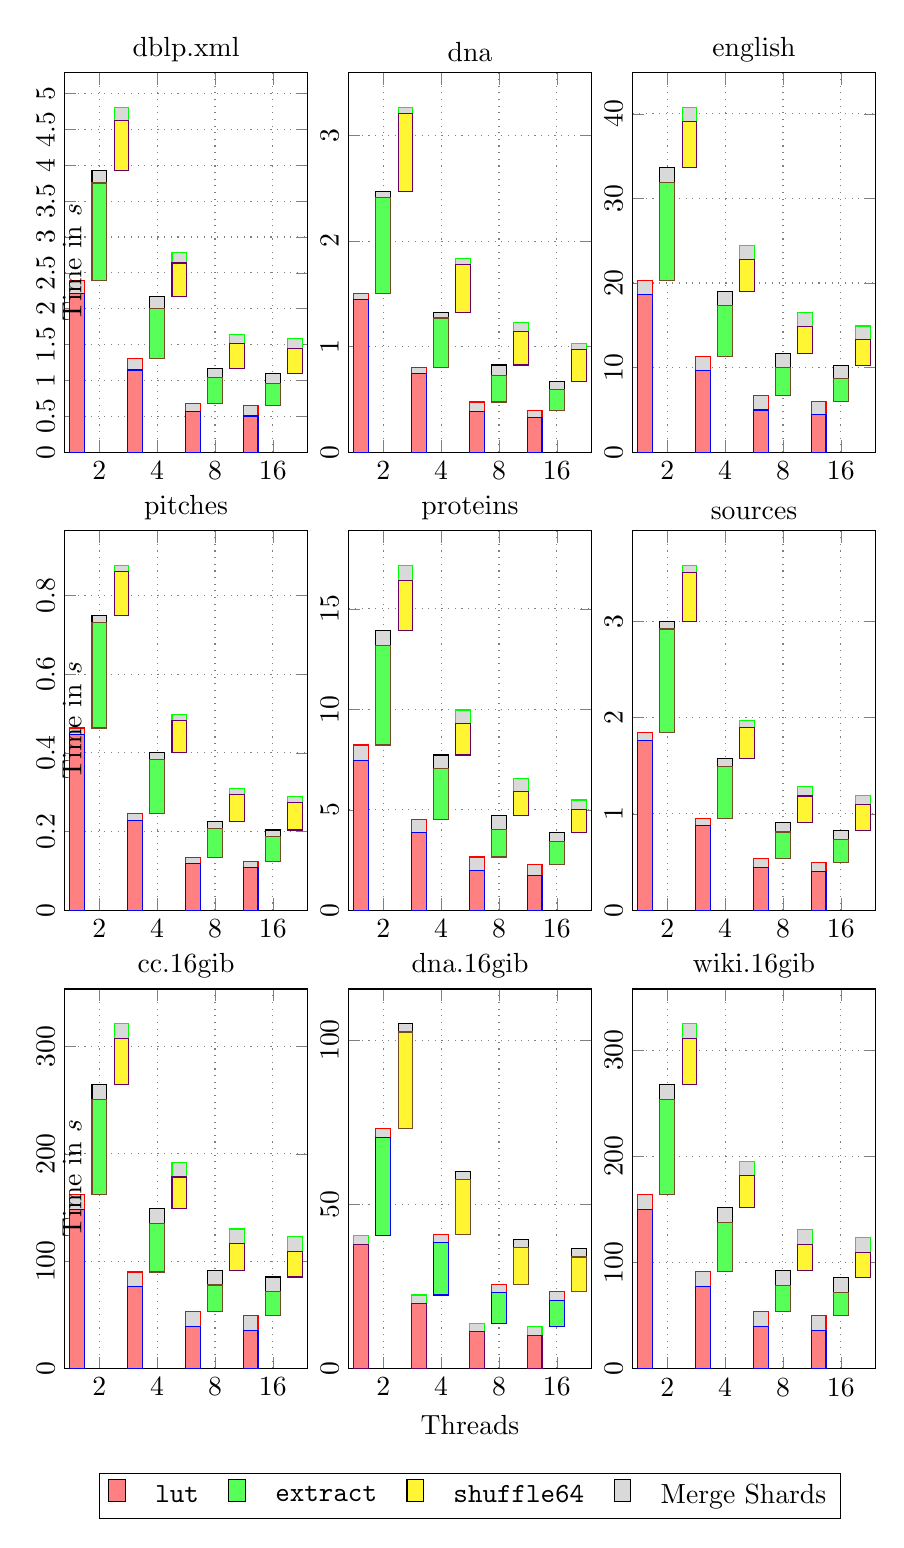
\begin{tikzpicture}
            \begin{groupplot} [
                ybar stacked,
                width = 0.385\textwidth,
                height = 6.4cm,
                enlarge x limits = 0.2,
                group style = { 
                    vertical sep = 1.0cm,
                    horizontal sep = 0.52cm,
                    group size = { 
                        3 by 3
                    } 
                },
                legend style = { 
                    at = {(0.5, -0.275)},
                    anchor = north,
                    legend columns = 4,
                    column sep = 2ex
                },
                yticklabel style = {
                    rotate = 90
                },
                ylabel style = {
                    at = {(0.11, 0.5)}
                },
                title style = {
                    at = {(0.5, 0.96)}
                },
                xticklabels = { , 1, 2, 4, 8, 16 },
                xtick distance = 1,
            ]
            
            
            \nextgroupplot [
                bar width = 0.185cm,
                title = dblp.xml,
                ylabel = Time in $s$,
                ytick distance = 0.5
            ]
    

            \resetplotddbreakdown{}
    
                %% PLOT SELECT LOG(2, threads) AS x, MEDIAN(ext_split) AS y
                %% FROM stats WHERE ((type LIKE 'lwtlut%')) AND (threads > 1) AND (file LIKE 'dblp.xml') GROUP BY x ORDER BY ds_order,x
                \addplot +[bar shift = -8pt, fill = red!50] coordinates { (1.0,2.21481) (2.0,1.14591) (3.0,0.562702) (4.0,0.503733) };

                %% PLOT SELECT LOG(2, threads) AS x, MEDIAN(time_in_s - ext_split) AS y
                %% FROM stats WHERE ((type LIKE 'lwtlut%')) AND (threads > 1) AND (file LIKE 'dblp.xml') GROUP BY x ORDER BY ds_order,x
                \addplot +[bar shift = -8pt, fill = black!15] coordinates { (1.0,0.18071) (2.0,0.16285) (3.0,0.11994) (4.0,0.144309) };
    
                \resetplotddbreakdown{}

                %% PLOT SELECT LOG(2, threads) AS x, MEDIAN(ext_split) AS y
                %% FROM stats WHERE ((type LIKE 'lwtpext%')) AND (threads > 1) AND (file LIKE 'dblp.xml') GROUP BY x ORDER BY ds_order,x
                \addplot +[bar shift = 0pt, fill = green!65] coordinates { (1.0,1.35828) (2.0,0.699003) (3.0,0.357627) (4.0,0.306109) };

                %% PLOT SELECT LOG(2, threads) AS x, MEDIAN(time_in_s - ext_split) AS y
                %% FROM stats WHERE ((type LIKE 'lwtpext%')) AND (threads > 1) AND (file LIKE 'dblp.xml') GROUP BY x ORDER BY ds_order,x
                \addplot +[bar shift = 0pt, fill = black!15] coordinates { (1.0,0.17485) (2.0,0.158407) (3.0,0.121524) (4.0,0.144416) };
    
                \resetplotddbreakdown{}

                %% PLOT SELECT LOG(2, threads) AS x, MEDIAN(ext_split) AS y
                %% FROM stats WHERE ((type LIKE 'lwtshuffle%')) AND (threads > 1) AND (file LIKE 'dblp.xml') GROUP BY x ORDER BY ds_order,x
                \addplot +[bar shift = 8pt, fill = yellow!80] coordinates { (1.0,0.701805) (2.0,0.47112) (3.0,0.350237) (4.0,0.341491) };

                %% PLOT SELECT LOG(2, threads) AS x, MEDIAN(time_in_s - ext_split) AS y
                %% FROM stats WHERE ((type LIKE 'lwtshuffle%')) AND (threads > 1) AND (file LIKE 'dblp.xml') GROUP BY x ORDER BY ds_order,x
                \addplot +[bar shift = 8pt, fill = black!15] coordinates { (1.0,0.181028) (2.0,0.143344) (3.0,0.126299) (4.0,0.143296) };
    
    
                \legend{};
    
       \nextgroupplot [
        ylabel = ,
        title = dna,
        bar width = 0.185cm
    ]
    
        
                %% PLOT SELECT LOG(2, threads) AS x, MEDIAN(ext_split) AS y
                %% FROM stats WHERE ((type LIKE 'lwtlut%')) AND (threads > 1) AND (file LIKE 'dna') GROUP BY x ORDER BY ds_order,x
                \addplot +[bar shift = -8pt, fill = red!50] coordinates { (1.0,1.44839) (2.0,0.741414) (3.0,0.383003) (4.0,0.33032) };

                %% PLOT SELECT LOG(2, threads) AS x, MEDIAN(time_in_s - ext_split) AS y
                %% FROM stats WHERE ((type LIKE 'lwtlut%')) AND (threads > 1) AND (file LIKE 'dna') GROUP BY x ORDER BY ds_order,x
                \addplot +[bar shift = -8pt, fill = black!15] coordinates { (1.0,0.05686) (2.0,0.056237) (3.0,0.091998) (4.0,0.063729) };
    
                \resetplotddbreakdown{}

                %% PLOT SELECT LOG(2, threads) AS x, MEDIAN(ext_split) AS y
                %% FROM stats WHERE ((type LIKE 'lwtpext%')) AND (threads > 1) AND (file LIKE 'dna') GROUP BY x ORDER BY ds_order,x
                \addplot +[bar shift = 0pt, fill = green!65] coordinates { (1.0,0.904998) (2.0,0.473228) (3.0,0.254779) (4.0,0.202585) };

                %% PLOT SELECT LOG(2, threads) AS x, MEDIAN(time_in_s - ext_split) AS y
                %% FROM stats WHERE ((type LIKE 'lwtpext%')) AND (threads > 1) AND (file LIKE 'dna') GROUP BY x ORDER BY ds_order,x
                \addplot +[bar shift = 0pt, fill = black!15] coordinates { (1.0,0.056939) (2.0,0.056111) (3.0,0.096172) (4.0,0.071204) };
    
                \resetplotddbreakdown{}

                %% PLOT SELECT LOG(2, threads) AS x, MEDIAN(ext_split) AS y
                %% FROM stats WHERE ((type LIKE 'lwtshuffle%')) AND (threads > 1) AND (file LIKE 'dna') GROUP BY x ORDER BY ds_order,x
                \addplot +[bar shift = 8pt, fill = yellow!80] coordinates { (1.0,0.744518) (2.0,0.450267) (3.0,0.31905) (4.0,0.301392) };

                %% PLOT SELECT LOG(2, threads) AS x, MEDIAN(time_in_s - ext_split) AS y
                %% FROM stats WHERE ((type LIKE 'lwtshuffle%')) AND (threads > 1) AND (file LIKE 'dna') GROUP BY x ORDER BY ds_order,x
                \addplot +[bar shift = 8pt, fill = black!15] coordinates { (1.0,0.056847) (2.0,0.05616) (3.0,0.084504) (4.0,0.063416) };
    
    
        \legend{};
    
    \nextgroupplot [
        ylabel = ,
        title = english,
        bar width = 0.185cm
    ]
    
                %% PLOT SELECT LOG(2, threads) AS x, MEDIAN(ext_split) AS y
                %% FROM stats WHERE ((type LIKE 'lwtlut%')) AND (threads > 1) AND (file LIKE 'english') GROUP BY x ORDER BY ds_order,x
                \addplot +[bar shift = -8pt, fill = red!50] coordinates { (1.0,18.6026) (2.0,9.62339) (3.0,4.98416) (4.0,4.48342) };

                %% PLOT SELECT LOG(2, threads) AS x, MEDIAN(time_in_s - ext_split) AS y
                %% FROM stats WHERE ((type LIKE 'lwtlut%')) AND (threads > 1) AND (file LIKE 'english') GROUP BY x ORDER BY ds_order,x
                \addplot +[bar shift = -8pt, fill = black!15] coordinates { (1.0,1.7047) (2.0,1.72955) (3.0,1.74014) (4.0,1.53324) };
    
                \resetplotddbreakdown{}

                %% PLOT SELECT LOG(2, threads) AS x, MEDIAN(ext_split) AS y
                %% FROM stats WHERE ((type LIKE 'lwtpext%')) AND (threads > 1) AND (file LIKE 'english') GROUP BY x ORDER BY ds_order,x
                \addplot +[bar shift = 0pt, fill = green!65] coordinates { (1.0,11.6026) (2.0,5.94552) (3.0,3.2395) (4.0,2.68211) };

                %% PLOT SELECT LOG(2, threads) AS x, MEDIAN(time_in_s - ext_split) AS y
                %% FROM stats WHERE ((type LIKE 'lwtpext%')) AND (threads > 1) AND (file LIKE 'english') GROUP BY x ORDER BY ds_order,x
                \addplot +[bar shift = 0pt, fill = black!15] coordinates { (1.0,1.7086) (2.0,1.72443) (3.0,1.74675) (4.0,1.55666) };
    
                \resetplotddbreakdown{}

                %% PLOT SELECT LOG(2, threads) AS x, MEDIAN(ext_split) AS y
                %% FROM stats WHERE ((type LIKE 'lwtshuffle%')) AND (threads > 1) AND (file LIKE 'english') GROUP BY x ORDER BY ds_order,x
                \addplot +[bar shift = 8pt, fill = yellow!80] coordinates { (1.0,5.46958) (2.0,3.7146) (3.0,3.10228) (4.0,3.09829) };

                %% PLOT SELECT LOG(2, threads) AS x, MEDIAN(time_in_s - ext_split) AS y
                %% FROM stats WHERE ((type LIKE 'lwtshuffle%')) AND (threads > 1) AND (file LIKE 'english') GROUP BY x ORDER BY ds_order,x
                \addplot +[bar shift = 8pt, fill = black!15] coordinates { (1.0,1.7048) (2.0,1.73615) (3.0,1.73546) (4.0,1.56094) };
    
    
        \legend{};
    
        \nextgroupplot [
        ylabel = Time in $s$,
        title = pitches,
        bar width = 0.185cm
    ]
    
                %% PLOT SELECT LOG(2, threads) AS x, MEDIAN(ext_split) AS y
                %% FROM stats WHERE ((type LIKE 'lwtlut%')) AND (threads > 1) AND (file LIKE 'pitches') GROUP BY x ORDER BY ds_order,x
                \addplot +[bar shift = -8pt, fill = red!50] coordinates { (1.0,0.446904) (2.0,0.22895) (3.0,0.118586) (4.0,0.107529) };

                %% PLOT SELECT LOG(2, threads) AS x, MEDIAN(time_in_s - ext_split) AS y
                %% FROM stats WHERE ((type LIKE 'lwtlut%')) AND (threads > 1) AND (file LIKE 'pitches') GROUP BY x ORDER BY ds_order,x
                \addplot +[bar shift = -8pt, fill = black!15] coordinates { (1.0,0.016466) (2.0,0.016241) (3.0,0.016119) (4.0,0.016275) };
    
                \resetplotddbreakdown{}

                %% PLOT SELECT LOG(2, threads) AS x, MEDIAN(ext_split) AS y
                %% FROM stats WHERE ((type LIKE 'lwtpext%')) AND (threads > 1) AND (file LIKE 'pitches') GROUP BY x ORDER BY ds_order,x
                \addplot +[bar shift = 0pt, fill = green!65] coordinates { (1.0,0.269061) (2.0,0.138761) (3.0,0.0740156) (4.0,0.0639577) };

                %% PLOT SELECT LOG(2, threads) AS x, MEDIAN(time_in_s - ext_split) AS y
                %% FROM stats WHERE ((type LIKE 'lwtpext%')) AND (threads > 1) AND (file LIKE 'pitches') GROUP BY x ORDER BY ds_order,x
                \addplot +[bar shift = 0pt, fill = black!15] coordinates { (1.0,0.016369) (2.0,0.015969) (3.0,0.0162259) (4.0,0.0163048) };
    
                \resetplotddbreakdown{}

                %% PLOT SELECT LOG(2, threads) AS x, MEDIAN(ext_split) AS y
                %% FROM stats WHERE ((type LIKE 'lwtshuffle%')) AND (threads > 1) AND (file LIKE 'pitches') GROUP BY x ORDER BY ds_order,x
                \addplot +[bar shift = 8pt, fill = yellow!80] coordinates { (1.0,0.111464) (2.0,0.08243) (3.0,0.069517) (4.0,0.0694285) };

                %% PLOT SELECT LOG(2, threads) AS x, MEDIAN(time_in_s - ext_split) AS y
                %% FROM stats WHERE ((type LIKE 'lwtshuffle%')) AND (threads > 1) AND (file LIKE 'pitches') GROUP BY x ORDER BY ds_order,x
                \addplot +[bar shift = 8pt, fill = black!15] coordinates { (1.0,0.016561) (2.0,0.0161251) (3.0,0.0161338) (4.0,0.0162842) };
    
    
                \legend{};
    
       \nextgroupplot [
        ylabel = ,
        title = proteins,
        bar width = 0.185cm
    ]
    
    
                %% PLOT SELECT LOG(2, threads) AS x, MEDIAN(ext_split) AS y
                %% FROM stats WHERE ((type LIKE 'lwtlut%')) AND (threads > 1) AND (file LIKE 'proteins') GROUP BY x ORDER BY ds_order,x
                \addplot +[bar shift = -8pt, fill = red!50] coordinates { (1.0,7.4732) (2.0,3.85244) (3.0,1.99016) (4.0,1.71889) };

                %% PLOT SELECT LOG(2, threads) AS x, MEDIAN(time_in_s - ext_split) AS y
                %% FROM stats WHERE ((type LIKE 'lwtlut%')) AND (threads > 1) AND (file LIKE 'proteins') GROUP BY x ORDER BY ds_order,x
                \addplot +[bar shift = -8pt, fill = black!15] coordinates { (1.0,0.75287) (2.0,0.66884) (3.0,0.65941) (4.0,0.54745) };
    
                \resetplotddbreakdown{}

                %% PLOT SELECT LOG(2, threads) AS x, MEDIAN(ext_split) AS y
                %% FROM stats WHERE ((type LIKE 'lwtpext%')) AND (threads > 1) AND (file LIKE 'proteins') GROUP BY x ORDER BY ds_order,x
                \addplot +[bar shift = 0pt, fill = green!65] coordinates { (1.0,4.94738) (2.0,2.54226) (3.0,1.38006) (4.0,1.13583) };

                %% PLOT SELECT LOG(2, threads) AS x, MEDIAN(time_in_s - ext_split) AS y
                %% FROM stats WHERE ((type LIKE 'lwtpext%')) AND (threads > 1) AND (file LIKE 'proteins') GROUP BY x ORDER BY ds_order,x
                \addplot +[bar shift = 0pt, fill = black!15] coordinates { (1.0,0.75242) (2.0,0.66522) (3.0,0.66723) (4.0,0.4694) };
    
                \resetplotddbreakdown{}

                %% PLOT SELECT LOG(2, threads) AS x, MEDIAN(ext_split) AS y
                %% FROM stats WHERE ((type LIKE 'lwtshuffle%')) AND (threads > 1) AND (file LIKE 'proteins') GROUP BY x ORDER BY ds_order,x
                \addplot +[bar shift = 8pt, fill = yellow!80] coordinates { (1.0,2.48712) (2.0,1.56663) (3.0,1.22764) (4.0,1.16369) };

                %% PLOT SELECT LOG(2, threads) AS x, MEDIAN(time_in_s - ext_split) AS y
                %% FROM stats WHERE ((type LIKE 'lwtshuffle%')) AND (threads > 1) AND (file LIKE 'proteins') GROUP BY x ORDER BY ds_order,x
                \addplot +[bar shift = 8pt, fill = black!15] coordinates { (1.0,0.75412) (2.0,0.67353) (3.0,0.65261) (4.0,0.45066) };
    
    
                \legend{};
    
    \nextgroupplot [
        ylabel = ,
        title = sources,
        bar width = 0.185cm
    ]
    
            %% PLOT SELECT LOG(2, threads) AS x, MEDIAN(ext_split) AS y
            %% FROM stats WHERE ((type LIKE 'lwtlut%')) AND (threads > 1) AND (file LIKE 'sources') GROUP BY x ORDER BY ds_order,x
            \addplot +[bar shift = -8pt, fill = red!50] coordinates { (1.0,1.76166) (2.0,0.875274) (3.0,0.439615) (4.0,0.403357) };

            %% PLOT SELECT LOG(2, threads) AS x, MEDIAN(time_in_s - ext_split) AS y
            %% FROM stats WHERE ((type LIKE 'lwtlut%')) AND (threads > 1) AND (file LIKE 'sources') GROUP BY x ORDER BY ds_order,x
            \addplot +[bar shift = -8pt, fill = black!15] coordinates { (1.0,0.07917) (2.0,0.077859) (3.0,0.095539) (4.0,0.091904) };

            \resetplotddbreakdown{}

            %% PLOT SELECT LOG(2, threads) AS x, MEDIAN(ext_split) AS y
            %% FROM stats WHERE ((type LIKE 'lwtpext%')) AND (threads > 1) AND (file LIKE 'sources') GROUP BY x ORDER BY ds_order,x
            \addplot +[bar shift = 0pt, fill = green!65] coordinates { (1.0,1.07898) (2.0,0.539853) (3.0,0.277194) (4.0,0.236793) };

            %% PLOT SELECT LOG(2, threads) AS x, MEDIAN(time_in_s - ext_split) AS y
            %% FROM stats WHERE ((type LIKE 'lwtpext%')) AND (threads > 1) AND (file LIKE 'sources') GROUP BY x ORDER BY ds_order,x
            \addplot +[bar shift = 0pt, fill = black!15] coordinates { (1.0,0.07922) (2.0,0.07806) (3.0,0.100316) (4.0,0.092087) };

            \resetplotddbreakdown{}

            %% PLOT SELECT LOG(2, threads) AS x, MEDIAN(ext_split) AS y
            %% FROM stats WHERE ((type LIKE 'lwtshuffle%')) AND (threads > 1) AND (file LIKE 'sources') GROUP BY x ORDER BY ds_order,x
            \addplot +[bar shift = 8pt, fill = yellow!80] coordinates { (1.0,0.505476) (2.0,0.327984) (3.0,0.273101) (4.0,0.273476) };

            %% PLOT SELECT LOG(2, threads) AS x, MEDIAN(time_in_s - ext_split) AS y
            %% FROM stats WHERE ((type LIKE 'lwtshuffle%')) AND (threads > 1) AND (file LIKE 'sources') GROUP BY x ORDER BY ds_order,x
            \addplot +[bar shift = 8pt, fill = black!15] coordinates { (1.0,0.075576) (2.0,0.074415) (3.0,0.100375) (4.0,0.097339) };


            \legend{};
        \nextgroupplot [
        ylabel = Time in $s$,
        bar width = 0.185cm,
        title = cc.16gib
    ]
    
    
                %% PLOT SELECT LOG(2, threads) AS x, MEDIAN(ext_split) AS y
                %% FROM stats WHERE ((type LIKE 'lwtlut%')) AND (threads > 1) AND (file LIKE 'cc.16gib') GROUP BY x ORDER BY ds_order,x
                \addplot +[bar shift = -8pt, fill = red!50] coordinates { (1.0,148.482) (2.0,76.1042) (3.0,39.4083) (4.0,35.6797) };

                %% PLOT SELECT LOG(2, threads) AS x, MEDIAN(time_in_s - ext_split) AS y
                %% FROM stats WHERE ((type LIKE 'lwtlut%')) AND (threads > 1) AND (file LIKE 'cc.16gib') GROUP BY x ORDER BY ds_order,x
                \addplot +[bar shift = -8pt, fill = black!15] coordinates { (1.0,13.901) (2.0,13.8126) (3.0,13.8576) (4.0,13.8545) };
    
                \resetplotddbreakdown{}

                %% PLOT SELECT LOG(2, threads) AS x, MEDIAN(ext_split) AS y
                %% FROM stats WHERE ((type LIKE 'lwtpext%')) AND (threads > 1) AND (file LIKE 'cc.16gib') GROUP BY x ORDER BY ds_order,x
                \addplot +[bar shift = 0pt, fill = green!65] coordinates { (1.0,88.1374) (2.0,44.9896) (3.0,24.4711) (4.0,21.776) };

                %% PLOT SELECT LOG(2, threads) AS x, MEDIAN(time_in_s - ext_split) AS y
                %% FROM stats WHERE ((type LIKE 'lwtpext%')) AND (threads > 1) AND (file LIKE 'cc.16gib') GROUP BY x ORDER BY ds_order,x
                \addplot +[bar shift = 0pt, fill = black!15] coordinates { (1.0,13.9222) (2.0,13.8205) (3.0,13.8874) (4.0,13.8741) };
    
                \resetplotddbreakdown{}

                %% PLOT SELECT LOG(2, threads) AS x, MEDIAN(ext_split) AS y
                %% FROM stats WHERE ((type LIKE 'lwtshuffle%')) AND (threads > 1) AND (file LIKE 'cc.16gib') GROUP BY x ORDER BY ds_order,x
                \addplot +[bar shift = 8pt, fill = yellow!80] coordinates { (1.0,43.4033) (2.0,29.7659) (3.0,24.5168) (4.0,24.1839) };

                %% PLOT SELECT LOG(2, threads) AS x, MEDIAN(time_in_s - ext_split) AS y
                %% FROM stats WHERE ((type LIKE 'lwtshuffle%')) AND (threads > 1) AND (file LIKE 'cc.16gib') GROUP BY x ORDER BY ds_order,x
                \addplot +[bar shift = 8pt, fill = black!15] coordinates { (1.0,13.8339) (2.0,13.8355) (3.0,13.8236) (4.0,13.8446) };
    
    
                \legend{};
    
    
       \nextgroupplot [
        xlabel = Threads,
        bar width = 0.185cm,
        title = dna.16gib
    ]
    
    \addplot [draw = none, fill = red!50] coordinates { (1,0) (2,0) (3,0) (4,0) };
    \addplot [draw = none, fill = green!65] coordinates { (1,0) (2,0) (3,0) (4,0) };
    \addplot [draw = none, fill = yellow!80] coordinates { (1,0) (2,0) (3,0) (4,0) };
    \addplot [draw = none, fill = black!15] coordinates { (1,0) (2,0) (3,0) (4,0) };


                %% PLOT SELECT LOG(2, threads) AS x, MEDIAN(ext_split) AS y
                %% FROM stats WHERE ((type LIKE 'lwtlut%')) AND (threads > 1) AND (file LIKE 'dna.16gib') GROUP BY x ORDER BY ds_order,x
                \addplot +[bar shift = -8pt, fill = red!50] coordinates { (1.0,37.8044) (2.0,19.7761) (3.0,11.1088) (4.0,10.0282) };

                %% PLOT SELECT LOG(2, threads) AS x, MEDIAN(time_in_s - ext_split) AS y
                %% FROM stats WHERE ((type LIKE 'lwtlut%')) AND (threads > 1) AND (file LIKE 'dna.16gib') GROUP BY x ORDER BY ds_order,x
                \addplot +[bar shift = -8pt, fill = black!15] coordinates { (1.0,2.5993) (2.0,2.5889) (3.0,2.6204) (4.0,2.62268) };
    
                \resetplotddbreakdown{}

                %% PLOT SELECT LOG(2, threads) AS x, MEDIAN(ext_split) AS y
                %% FROM stats WHERE ((type LIKE 'lwtpext%')) AND (threads > 1) AND (file LIKE 'dna.16gib') GROUP BY x ORDER BY ds_order,x
                \addplot +[bar shift = 0pt, fill = green!65] coordinates { (1.0,30.0191) (2.0,15.9022) (3.0,9.26073) (4.0,8.10458) };

                %% PLOT SELECT LOG(2, threads) AS x, MEDIAN(time_in_s - ext_split) AS y
                %% FROM stats WHERE ((type LIKE 'lwtpext%')) AND (threads > 1) AND (file LIKE 'dna.16gib') GROUP BY x ORDER BY ds_order,x
                \addplot +[bar shift = 0pt, fill = black!15] coordinates { (1.0,2.6001) (2.0,2.5875) (3.0,2.62476) (4.0,2.63309) };
    
                \resetplotddbreakdown{}

                %% PLOT SELECT LOG(2, threads) AS x, MEDIAN(ext_split) AS y
                %% FROM stats WHERE ((type LIKE 'lwtshuffle%')) AND (threads > 1) AND (file LIKE 'dna.16gib') GROUP BY x ORDER BY ds_order,x
                \addplot +[bar shift = 8pt, fill = yellow!80] coordinates { (1.0,29.4325) (2.0,16.5599) (3.0,11.1651) (4.0,10.5437) };

                %% PLOT SELECT LOG(2, threads) AS x, MEDIAN(time_in_s - ext_split) AS y
                %% FROM stats WHERE ((type LIKE 'lwtshuffle%')) AND (threads > 1) AND (file LIKE 'dna.16gib') GROUP BY x ORDER BY ds_order,x
                \addplot +[bar shift = 8pt, fill = black!15] coordinates { (1.0,2.6016) (2.0,2.586) (3.0,2.6055) (4.0,2.6137) };

    
        \legend{
            \texttt{lut},
            \texttt{extract},
            \texttt{shuffle64},
            Merge Shards
        };
    
    \nextgroupplot [
        ylabel = ,
        bar width = 0.185cm,
        title = wiki.16gib
    ]
    
                %% PLOT SELECT LOG(2, threads) AS x, MEDIAN(ext_split) AS y
                %% FROM stats WHERE ((type LIKE 'lwtlut%')) AND (threads > 1) AND (file LIKE 'wiki.16gib') GROUP BY x ORDER BY ds_order,x
                \addplot +[bar shift = -8pt, fill = red!50] coordinates { (1.0,149.699) (2.0,77.3314) (3.0,39.7704) (4.0,35.8444) };

                %% PLOT SELECT LOG(2, threads) AS x, MEDIAN(time_in_s - ext_split) AS y
                %% FROM stats WHERE ((type LIKE 'lwtlut%')) AND (threads > 1) AND (file LIKE 'wiki.16gib') GROUP BY x ORDER BY ds_order,x
                \addplot +[bar shift = -8pt, fill = black!15] coordinates { (1.0,13.814) (2.0,13.8605) (3.0,13.8683) (4.0,13.8636) };
    
                \resetplotddbreakdown{}

                %% PLOT SELECT LOG(2, threads) AS x, MEDIAN(ext_split) AS y
                %% FROM stats WHERE ((type LIKE 'lwtpext%')) AND (threads > 1) AND (file LIKE 'wiki.16gib') GROUP BY x ORDER BY ds_order,x
                \addplot +[bar shift = 0pt, fill = green!65] coordinates { (1.0,90.0777) (2.0,46.5589) (3.0,24.7826) (4.0,21.8503) };

                %% PLOT SELECT LOG(2, threads) AS x, MEDIAN(time_in_s - ext_split) AS y
                %% FROM stats WHERE ((type LIKE 'lwtpext%')) AND (threads > 1) AND (file LIKE 'wiki.16gib') GROUP BY x ORDER BY ds_order,x
                \addplot +[bar shift = 0pt, fill = black!15] coordinates { (1.0,13.9277) (2.0,13.8218) (3.0,13.862) (4.0,13.8621) };
    
                \resetplotddbreakdown{}

                %% PLOT SELECT LOG(2, threads) AS x, MEDIAN(ext_split) AS y
                %% FROM stats WHERE ((type LIKE 'lwtshuffle%')) AND (threads > 1) AND (file LIKE 'wiki.16gib') GROUP BY x ORDER BY ds_order,x
                \addplot +[bar shift = 8pt, fill = yellow!80] coordinates { (1.0,43.8156) (2.0,29.845) (3.0,24.4358) (4.0,24.2443) };

                %% PLOT SELECT LOG(2, threads) AS x, MEDIAN(time_in_s - ext_split) AS y
                %% FROM stats WHERE ((type LIKE 'lwtshuffle%')) AND (threads > 1) AND (file LIKE 'wiki.16gib') GROUP BY x ORDER BY ds_order,x
                \addplot +[bar shift = 8pt, fill = black!15] coordinates { (1.0,13.7832) (2.0,13.9654) (3.0,13.825) (4.0,13.8196) };
    
    
                \legend{};
            \end{groupplot}
            \end{tikzpicture}
        \end{center}
    \caption{
        We break down the construction time in seconds of our domain decomposition algorithms.
        The time spent merging all slices is shown in grey.
        As can be seen, the time spent merging largely not affected by the number of threads.
    }
    \label{fig:eval-dd-texts-breakdown-wt}
    \end{figure}    

\clearpage 

\begin{figure}[t]
    \begin{center}
        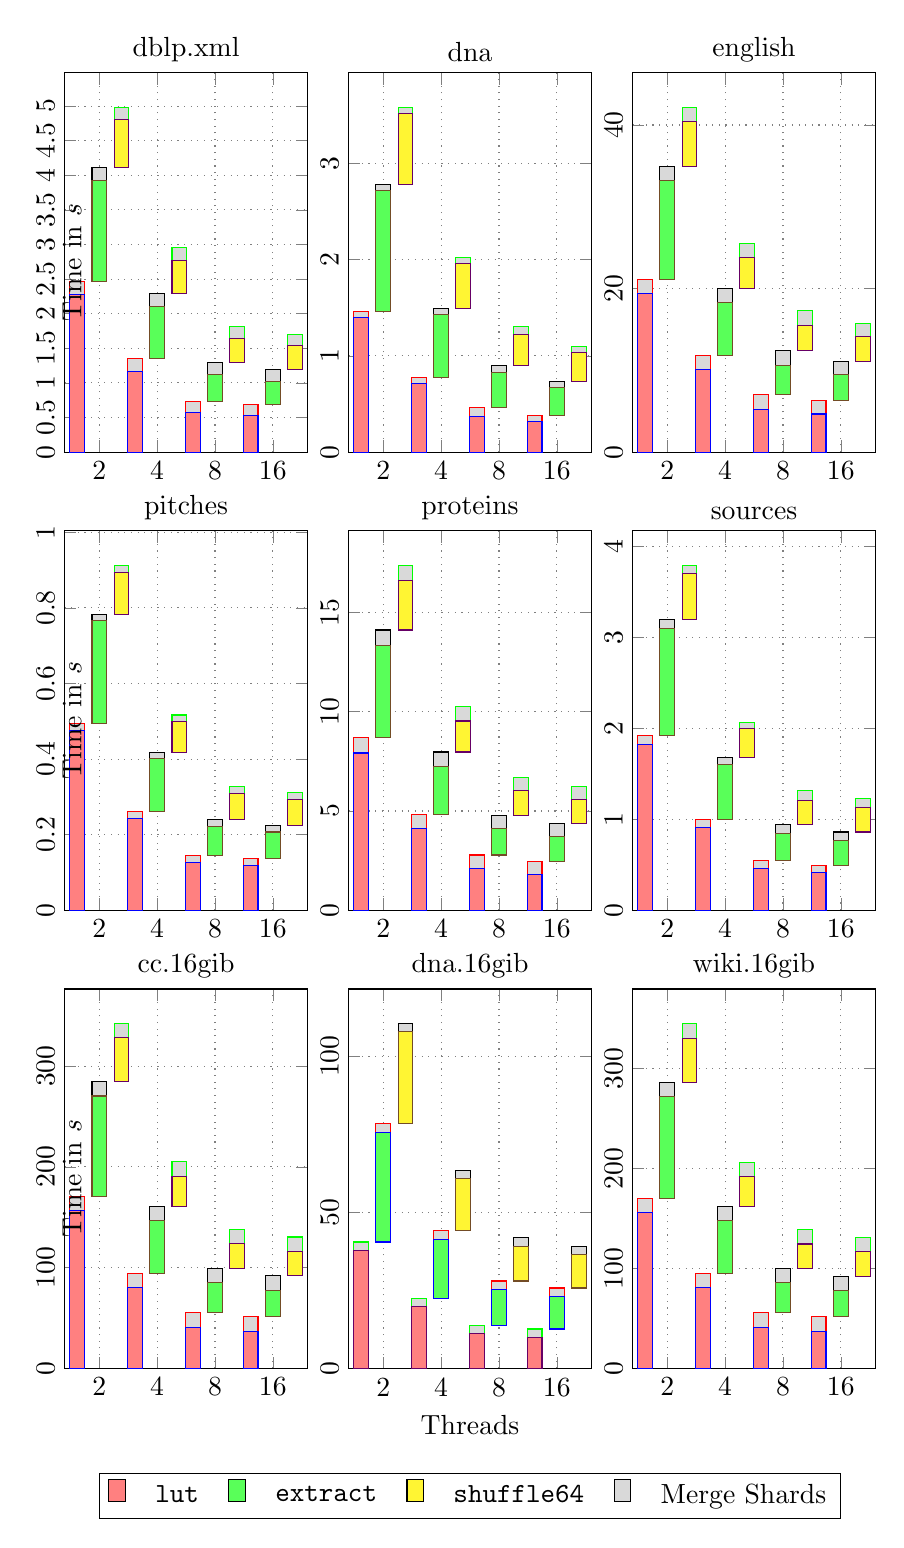
\begin{tikzpicture}
            \begin{groupplot} [
                ybar stacked,
                width = 0.385\textwidth,
                height = 6.4cm,
                enlarge x limits = 0.2,
                group style = { 
                    vertical sep = 1.0cm,
                    horizontal sep = 0.52cm,
                    group size = { 
                        3 by 3
                    } 
                },
                legend style = { 
                    at = {(0.5, -0.275)},
                    anchor = north,
                    legend columns = 4,
                    column sep = 2ex
                },
                yticklabel style = {
                    rotate = 90
                },
                ylabel style = {
                    at = {(0.11, 0.5)}
                },
                title style = {
                    at = {(0.5, 0.96)}
                },
                xticklabels = { , 1, 2, 4, 8, 16 },
                xtick distance = 1,
            ]
            
            
            \nextgroupplot [
                bar width = 0.185cm,
                title = dblp.xml,
                ylabel = Time in $s$,
                ytick distance = 0.5
            ]
    

            \resetplotddbreakdown{}
    
                %% PLOT SELECT LOG(2, threads) AS x, MEDIAN(ext_split) AS y
                %% FROM stats WHERE ((type LIKE 'wmlut%')) AND (threads > 1) AND (file LIKE 'dblp.xml') GROUP BY x ORDER BY ds_order,x
                \addplot +[bar shift = -8pt, fill = red!50] coordinates { (1.0,2.28137) (2.0,1.16788) (3.0,0.576258) (4.0,0.524412) };

                %% PLOT SELECT LOG(2, threads) AS x, MEDIAN(time_in_s - ext_split) AS y
                %% FROM stats WHERE ((type LIKE 'wmlut%')) AND (threads > 1) AND (file LIKE 'dblp.xml') GROUP BY x ORDER BY ds_order,x
                \addplot +[bar shift = -8pt, fill = black!15] coordinates { (1.0,0.18036) (2.0,0.18099) (3.0,0.156706) (4.0,0.1679) };
    
                \resetplotddbreakdown{}

                %% PLOT SELECT LOG(2, threads) AS x, MEDIAN(ext_split) AS y
                %% FROM stats WHERE ((type LIKE 'wmpext%')) AND (threads > 1) AND (file LIKE 'dblp.xml') GROUP BY x ORDER BY ds_order,x
                \addplot +[bar shift = 0pt, fill = green!65] coordinates { (1.0,1.46809) (2.0,0.759971) (3.0,0.394742) (4.0,0.332946) };

                %% PLOT SELECT LOG(2, threads) AS x, MEDIAN(time_in_s - ext_split) AS y
                %% FROM stats WHERE ((type LIKE 'wmpext%')) AND (threads > 1) AND (file LIKE 'dblp.xml') GROUP BY x ORDER BY ds_order,x
                \addplot +[bar shift = 0pt, fill = black!15] coordinates { (1.0,0.17634) (2.0,0.186663) (3.0,0.168156) (4.0,0.16956) };
    
                \resetplotddbreakdown{}

                %% PLOT SELECT LOG(2, threads) AS x, MEDIAN(ext_split) AS y
                %% FROM stats WHERE ((type LIKE 'wmshuffle%')) AND (threads > 1) AND (file LIKE 'dblp.xml') GROUP BY x ORDER BY ds_order,x
                \addplot +[bar shift = 8pt, fill = yellow!80] coordinates { (1.0,0.69916) (2.0,0.471298) (3.0,0.346693) (4.0,0.340359) };

                %% PLOT SELECT LOG(2, threads) AS x, MEDIAN(time_in_s - ext_split) AS y
                %% FROM stats WHERE ((type LIKE 'wmshuffle%')) AND (threads > 1) AND (file LIKE 'dblp.xml') GROUP BY x ORDER BY ds_order,x
                \addplot +[bar shift = 8pt, fill = black!15] coordinates { (1.0,0.178436) (2.0,0.184135) (3.0,0.166979) (4.0,0.162656) };
    
    
                \legend{};
    
       \nextgroupplot [
        ylabel = ,
        title = dna,
        bar width = 0.185cm
    ]
    
        
                %% PLOT SELECT LOG(2, threads) AS x, MEDIAN(ext_split) AS y
                %% FROM stats WHERE ((type LIKE 'wmlut%')) AND (threads > 1) AND (file LIKE 'dna') GROUP BY x ORDER BY ds_order,x
                \addplot +[bar shift = -8pt, fill = red!50] coordinates { (1.0,1.40263) (2.0,0.712452) (3.0,0.366893) (4.0,0.321709) };

                %% PLOT SELECT LOG(2, threads) AS x, MEDIAN(time_in_s - ext_split) AS y
                %% FROM stats WHERE ((type LIKE 'wmlut%')) AND (threads > 1) AND (file LIKE 'dna') GROUP BY x ORDER BY ds_order,x
                \addplot +[bar shift = -8pt, fill = black!15] coordinates { (1.0,0.06143) (2.0,0.060736) (3.0,0.099605) (4.0,0.061195) };
    
                \resetplotddbreakdown{}

                %% PLOT SELECT LOG(2, threads) AS x, MEDIAN(ext_split) AS y
                %% FROM stats WHERE ((type LIKE 'wmpext%')) AND (threads > 1) AND (file LIKE 'dna') GROUP BY x ORDER BY ds_order,x
                \addplot +[bar shift = 0pt, fill = green!65] coordinates { (1.0,1.25285) (2.0,0.65457) (3.0,0.361342) (4.0,0.286335) };

                %% PLOT SELECT LOG(2, threads) AS x, MEDIAN(time_in_s - ext_split) AS y
                %% FROM stats WHERE ((type LIKE 'wmpext%')) AND (threads > 1) AND (file LIKE 'dna') GROUP BY x ORDER BY ds_order,x
                \addplot +[bar shift = 0pt, fill = black!15] coordinates { (1.0,0.06141) (2.0,0.060796) (3.0,0.076281) (4.0,0.061292) };
    
                \resetplotddbreakdown{}

                %% PLOT SELECT LOG(2, threads) AS x, MEDIAN(ext_split) AS y
                %% FROM stats WHERE ((type LIKE 'wmshuffle%')) AND (threads > 1) AND (file LIKE 'dna') GROUP BY x ORDER BY ds_order,x
                \addplot +[bar shift = 8pt, fill = yellow!80] coordinates { (1.0,0.744288) (2.0,0.468825) (3.0,0.314527) (4.0,0.303747) };

                %% PLOT SELECT LOG(2, threads) AS x, MEDIAN(time_in_s - ext_split) AS y
                %% FROM stats WHERE ((type LIKE 'wmshuffle%')) AND (threads > 1) AND (file LIKE 'dna') GROUP BY x ORDER BY ds_order,x
                \addplot +[bar shift = 8pt, fill = black!15] coordinates { (1.0,0.06155) (2.0,0.060779) (3.0,0.085974) (4.0,0.061322) };
    
    
        \legend{};
    
    \nextgroupplot [
        ylabel = ,
        title = english,
        bar width = 0.185cm
    ]
    
                %% PLOT SELECT LOG(2, threads) AS x, MEDIAN(ext_split) AS y
                %% FROM stats WHERE ((type LIKE 'wmlut%')) AND (threads > 1) AND (file LIKE 'english') GROUP BY x ORDER BY ds_order,x
                \addplot +[bar shift = -8pt, fill = red!50] coordinates { (1.0,19.347) (2.0,10.0768) (3.0,5.22277) (4.0,4.65615) };

                %% PLOT SELECT LOG(2, threads) AS x, MEDIAN(time_in_s - ext_split) AS y
                %% FROM stats WHERE ((type LIKE 'wmlut%')) AND (threads > 1) AND (file LIKE 'english') GROUP BY x ORDER BY ds_order,x
                \addplot +[bar shift = -8pt, fill = black!15] coordinates { (1.0,1.763) (2.0,1.781) (3.0,1.79961) (4.0,1.63332) };
    
                \resetplotddbreakdown{}

                %% PLOT SELECT LOG(2, threads) AS x, MEDIAN(ext_split) AS y
                %% FROM stats WHERE ((type LIKE 'wmpext%')) AND (threads > 1) AND (file LIKE 'english') GROUP BY x ORDER BY ds_order,x
                \addplot +[bar shift = 0pt, fill = green!65] coordinates { (1.0,12.0755) (2.0,6.41742) (3.0,3.55811) (4.0,3.16809) };

                %% PLOT SELECT LOG(2, threads) AS x, MEDIAN(time_in_s - ext_split) AS y
                %% FROM stats WHERE ((type LIKE 'wmpext%')) AND (threads > 1) AND (file LIKE 'english') GROUP BY x ORDER BY ds_order,x
                \addplot +[bar shift = 0pt, fill = black!15] coordinates { (1.0,1.7607) (2.0,1.77908) (3.0,1.79716) (4.0,1.6088) };
    
                \resetplotddbreakdown{}

                %% PLOT SELECT LOG(2, threads) AS x, MEDIAN(ext_split) AS y
                %% FROM stats WHERE ((type LIKE 'wmshuffle%')) AND (threads > 1) AND (file LIKE 'english') GROUP BY x ORDER BY ds_order,x
                \addplot +[bar shift = 8pt, fill = yellow!80] coordinates { (1.0,5.46518) (2.0,3.71641) (3.0,3.10581) (4.0,3.08711) };

                %% PLOT SELECT LOG(2, threads) AS x, MEDIAN(time_in_s - ext_split) AS y
                %% FROM stats WHERE ((type LIKE 'wmshuffle%')) AND (threads > 1) AND (file LIKE 'english') GROUP BY x ORDER BY ds_order,x
                \addplot +[bar shift = 8pt, fill = black!15] coordinates { (1.0,1.77148) (2.0,1.78194) (3.0,1.78994) (4.0,1.60876) };
    
    
        \legend{};
    
        \nextgroupplot [
        ylabel = Time in $s$,
        title = pitches,
        bar width = 0.185cm
    ]
    
                %% PLOT SELECT LOG(2, threads) AS x, MEDIAN(ext_split) AS y
                %% FROM stats WHERE ((type LIKE 'wmlut%')) AND (threads > 1) AND (file LIKE 'pitches') GROUP BY x ORDER BY ds_order,x
                \addplot +[bar shift = -8pt, fill = red!50] coordinates { (1.0,0.476105) (2.0,0.242802) (3.0,0.126853) (4.0,0.119039) };

                %% PLOT SELECT LOG(2, threads) AS x, MEDIAN(time_in_s - ext_split) AS y
                %% FROM stats WHERE ((type LIKE 'wmlut%')) AND (threads > 1) AND (file LIKE 'pitches') GROUP BY x ORDER BY ds_order,x
                \addplot +[bar shift = -8pt, fill = black!15] coordinates { (1.0,0.017794) (2.0,0.017562) (3.0,0.017703) (4.0,0.017871) };
    
                \resetplotddbreakdown{}

                %% PLOT SELECT LOG(2, threads) AS x, MEDIAN(ext_split) AS y
                %% FROM stats WHERE ((type LIKE 'wmpext%')) AND (threads > 1) AND (file LIKE 'pitches') GROUP BY x ORDER BY ds_order,x
                \addplot +[bar shift = 0pt, fill = green!65] coordinates { (1.0,0.271808) (2.0,0.140388) (3.0,0.0772457) (4.0,0.0700075) };

                %% PLOT SELECT LOG(2, threads) AS x, MEDIAN(time_in_s - ext_split) AS y
                %% FROM stats WHERE ((type LIKE 'wmpext%')) AND (threads > 1) AND (file LIKE 'pitches') GROUP BY x ORDER BY ds_order,x
                \addplot +[bar shift = 0pt, fill = black!15] coordinates { (1.0,0.017945) (2.0,0.01745) (3.0,0.0177122) (4.0,0.0178482) };
    
                \resetplotddbreakdown{}

                %% PLOT SELECT LOG(2, threads) AS x, MEDIAN(ext_split) AS y
                %% FROM stats WHERE ((type LIKE 'wmshuffle%')) AND (threads > 1) AND (file LIKE 'pitches') GROUP BY x ORDER BY ds_order,x
                \addplot +[bar shift = 8pt, fill = yellow!80] coordinates { (1.0,0.111036) (2.0,0.0809824) (3.0,0.0691469) (4.0,0.0693768) };

                %% PLOT SELECT LOG(2, threads) AS x, MEDIAN(time_in_s - ext_split) AS y
                %% FROM stats WHERE ((type LIKE 'wmshuffle%')) AND (threads > 1) AND (file LIKE 'pitches') GROUP BY x ORDER BY ds_order,x
                \addplot +[bar shift = 8pt, fill = black!15] coordinates { (1.0,0.01794) (2.0,0.0175681) (3.0,0.0177083) (4.0,0.0178859) };
    
    
                \legend{};
    
       \nextgroupplot [
        ylabel = ,
        title = proteins,
        bar width = 0.185cm
    ]
    
    
                %% PLOT SELECT LOG(2, threads) AS x, MEDIAN(ext_split) AS y
                %% FROM stats WHERE ((type LIKE 'wmlut%')) AND (threads > 1) AND (file LIKE 'proteins') GROUP BY x ORDER BY ds_order,x
                \addplot +[bar shift = -8pt, fill = red!50] coordinates { (1.0,7.92334) (2.0,4.13043) (3.0,2.11333) (4.0,1.81698) };

                %% PLOT SELECT LOG(2, threads) AS x, MEDIAN(time_in_s - ext_split) AS y
                %% FROM stats WHERE ((type LIKE 'wmlut%')) AND (threads > 1) AND (file LIKE 'proteins') GROUP BY x ORDER BY ds_order,x
                \addplot +[bar shift = -8pt, fill = black!15] coordinates { (1.0,0.77171) (2.0,0.70782) (3.0,0.67035) (4.0,0.65585) };
    
                \resetplotddbreakdown{}

                %% PLOT SELECT LOG(2, threads) AS x, MEDIAN(ext_split) AS y
                %% FROM stats WHERE ((type LIKE 'wmpext%')) AND (threads > 1) AND (file LIKE 'proteins') GROUP BY x ORDER BY ds_order,x
                \addplot +[bar shift = 0pt, fill = green!65] coordinates { (1.0,4.65058) (2.0,2.4198) (3.0,1.32716) (4.0,1.22783) };

                %% PLOT SELECT LOG(2, threads) AS x, MEDIAN(time_in_s - ext_split) AS y
                %% FROM stats WHERE ((type LIKE 'wmpext%')) AND (threads > 1) AND (file LIKE 'proteins') GROUP BY x ORDER BY ds_order,x
                \addplot +[bar shift = 0pt, fill = black!15] coordinates { (1.0,0.77384) (2.0,0.71215) (3.0,0.67446) (4.0,0.65586) };
    
                \resetplotddbreakdown{}

                %% PLOT SELECT LOG(2, threads) AS x, MEDIAN(ext_split) AS y
                %% FROM stats WHERE ((type LIKE 'wmshuffle%')) AND (threads > 1) AND (file LIKE 'proteins') GROUP BY x ORDER BY ds_order,x
                \addplot +[bar shift = 8pt, fill = yellow!80] coordinates { (1.0,2.48348) (2.0,1.5634) (3.0,1.24302) (4.0,1.21707) };

                %% PLOT SELECT LOG(2, threads) AS x, MEDIAN(time_in_s - ext_split) AS y
                %% FROM stats WHERE ((type LIKE 'wmshuffle%')) AND (threads > 1) AND (file LIKE 'proteins') GROUP BY x ORDER BY ds_order,x
                \addplot +[bar shift = 8pt, fill = black!15] coordinates { (1.0,0.77135) (2.0,0.71167) (3.0,0.67043) (4.0,0.6572) };
    
    
                \legend{};
    
    \nextgroupplot [
        ylabel = ,
        title = sources,
        bar width = 0.185cm
    ]
    
            %% PLOT SELECT LOG(2, threads) AS x, MEDIAN(ext_split) AS y
            %% FROM stats WHERE ((type LIKE 'wmlut%')) AND (threads > 1) AND (file LIKE 'sources') GROUP BY x ORDER BY ds_order,x
            \addplot +[bar shift = -8pt, fill = red!50] coordinates { (1.0,1.82079) (2.0,0.906934) (3.0,0.454509) (4.0,0.417729) };

            %% PLOT SELECT LOG(2, threads) AS x, MEDIAN(time_in_s - ext_split) AS y
            %% FROM stats WHERE ((type LIKE 'wmlut%')) AND (threads > 1) AND (file LIKE 'sources') GROUP BY x ORDER BY ds_order,x
            \addplot +[bar shift = -8pt, fill = black!15] coordinates { (1.0,0.09682) (2.0,0.089418) (3.0,0.09003) (4.0,0.076855) };

            \resetplotddbreakdown{}

            %% PLOT SELECT LOG(2, threads) AS x, MEDIAN(ext_split) AS y
            %% FROM stats WHERE ((type LIKE 'wmpext%')) AND (threads > 1) AND (file LIKE 'sources') GROUP BY x ORDER BY ds_order,x
            \addplot +[bar shift = 0pt, fill = green!65] coordinates { (1.0,1.18427) (2.0,0.608297) (3.0,0.303707) (4.0,0.273021) };

            %% PLOT SELECT LOG(2, threads) AS x, MEDIAN(time_in_s - ext_split) AS y
            %% FROM stats WHERE ((type LIKE 'wmpext%')) AND (threads > 1) AND (file LIKE 'sources') GROUP BY x ORDER BY ds_order,x
            \addplot +[bar shift = 0pt, fill = black!15] coordinates { (1.0,0.09092) (2.0,0.07104) (3.0,0.093316) (4.0,0.092622) };

            \resetplotddbreakdown{}

            %% PLOT SELECT LOG(2, threads) AS x, MEDIAN(ext_split) AS y
            %% FROM stats WHERE ((type LIKE 'wmshuffle%')) AND (threads > 1) AND (file LIKE 'sources') GROUP BY x ORDER BY ds_order,x
            \addplot +[bar shift = 8pt, fill = yellow!80] coordinates { (1.0,0.50646) (2.0,0.319976) (3.0,0.268258) (4.0,0.2696) };

            %% PLOT SELECT LOG(2, threads) AS x, MEDIAN(time_in_s - ext_split) AS y
            %% FROM stats WHERE ((type LIKE 'wmshuffle%')) AND (threads > 1) AND (file LIKE 'sources') GROUP BY x ORDER BY ds_order,x
            \addplot +[bar shift = 8pt, fill = black!15] coordinates { (1.0,0.092346) (2.0,0.06911) (3.0,0.105523) (4.0,0.101378) };


            \legend{};
        \nextgroupplot [
        ylabel = Time in $s$,
        bar width = 0.185cm,
        title = cc.16gib
    ]
    
    
                %% PLOT SELECT LOG(2, threads) AS x, MEDIAN(ext_split) AS y
                %% FROM stats WHERE ((type LIKE 'wmlut%')) AND (threads > 1) AND (file LIKE 'cc.16gib') GROUP BY x ORDER BY ds_order,x
                \addplot +[bar shift = -8pt, fill = red!50] coordinates { (1.0,156.32) (2.0,80.1529) (3.0,41.0191) (4.0,37.0316) };

                %% PLOT SELECT LOG(2, threads) AS x, MEDIAN(time_in_s - ext_split) AS y
                %% FROM stats WHERE ((type LIKE 'wmlut%')) AND (threads > 1) AND (file LIKE 'cc.16gib') GROUP BY x ORDER BY ds_order,x
                \addplot +[bar shift = -8pt, fill = black!15] coordinates { (1.0,14.355) (2.0,14.2367) (3.0,14.3234) (4.0,14.3353) };
    
                \resetplotddbreakdown{}

                %% PLOT SELECT LOG(2, threads) AS x, MEDIAN(ext_split) AS y
                %% FROM stats WHERE ((type LIKE 'wmpext%')) AND (threads > 1) AND (file LIKE 'cc.16gib') GROUP BY x ORDER BY ds_order,x
                \addplot +[bar shift = 0pt, fill = green!65] coordinates { (1.0,99.6382) (2.0,52.1218) (3.0,29.502) (4.0,26.0296) };

                %% PLOT SELECT LOG(2, threads) AS x, MEDIAN(time_in_s - ext_split) AS y
                %% FROM stats WHERE ((type LIKE 'wmpext%')) AND (threads > 1) AND (file LIKE 'cc.16gib') GROUP BY x ORDER BY ds_order,x
                \addplot +[bar shift = 0pt, fill = black!15] coordinates { (1.0,14.3346) (2.0,14.5697) (3.0,14.347) (4.0,14.5374) };
    
                \resetplotddbreakdown{}

                %% PLOT SELECT LOG(2, threads) AS x, MEDIAN(ext_split) AS y
                %% FROM stats WHERE ((type LIKE 'wmshuffle%')) AND (threads > 1) AND (file LIKE 'cc.16gib') GROUP BY x ORDER BY ds_order,x
                \addplot +[bar shift = 8pt, fill = yellow!80] coordinates { (1.0,43.3865) (2.0,29.7458) (3.0,24.394) (4.0,24.1221) };

                %% PLOT SELECT LOG(2, threads) AS x, MEDIAN(time_in_s - ext_split) AS y
                %% FROM stats WHERE ((type LIKE 'wmshuffle%')) AND (threads > 1) AND (file LIKE 'cc.16gib') GROUP BY x ORDER BY ds_order,x
                \addplot +[bar shift = 8pt, fill = black!15] coordinates { (1.0,14.2496) (2.0,14.232) (3.0,14.3087) (4.0,14.2877) };
    
    
                \legend{};
    
    
       \nextgroupplot [
        xlabel = Threads,
        bar width = 0.185cm,
        title = dna.16gib
    ]
    
    \addplot [draw = none, fill = red!50] coordinates { (1,0) (2,0) (3,0) (4,0) };
    \addplot [draw = none, fill = green!65] coordinates { (1,0) (2,0) (3,0) (4,0) };
    \addplot [draw = none, fill = yellow!80] coordinates { (1,0) (2,0) (3,0) (4,0) };
    \addplot [draw = none, fill = black!15] coordinates { (1,0) (2,0) (3,0) (4,0) };


                %% PLOT SELECT LOG(2, threads) AS x, MEDIAN(ext_split) AS y
                %% FROM stats WHERE ((type LIKE 'wmlut%')) AND (threads > 1) AND (file LIKE 'dna.16gib') GROUP BY x ORDER BY ds_order,x
                \addplot +[bar shift = -8pt, fill = red!50] coordinates { (1.0,37.8176) (2.0,19.8355) (3.0,11.0838) (4.0,9.93173) };

                %% PLOT SELECT LOG(2, threads) AS x, MEDIAN(time_in_s - ext_split) AS y
                %% FROM stats WHERE ((type LIKE 'wmlut%')) AND (threads > 1) AND (file LIKE 'dna.16gib') GROUP BY x ORDER BY ds_order,x
                \addplot +[bar shift = -8pt, fill = black!15] coordinates { (1.0,2.6659) (2.0,2.6507) (3.0,2.683) (4.0,2.69089) };
    
                \resetplotddbreakdown{}

                %% PLOT SELECT LOG(2, threads) AS x, MEDIAN(ext_split) AS y
                %% FROM stats WHERE ((type LIKE 'wmpext%')) AND (threads > 1) AND (file LIKE 'dna.16gib') GROUP BY x ORDER BY ds_order,x
                \addplot +[bar shift = 0pt, fill = green!65] coordinates { (1.0,35.2035) (2.0,18.9316) (3.0,11.5314) (4.0,10.4104) };

                %% PLOT SELECT LOG(2, threads) AS x, MEDIAN(time_in_s - ext_split) AS y
                %% FROM stats WHERE ((type LIKE 'wmpext%')) AND (threads > 1) AND (file LIKE 'dna.16gib') GROUP BY x ORDER BY ds_order,x
                \addplot +[bar shift = 0pt, fill = black!15] coordinates { (1.0,2.6756) (2.0,2.6474) (3.0,2.6952) (4.0,2.7051) };
    
                \resetplotddbreakdown{}

                %% PLOT SELECT LOG(2, threads) AS x, MEDIAN(ext_split) AS y
                %% FROM stats WHERE ((type LIKE 'wmshuffle%')) AND (threads > 1) AND (file LIKE 'dna.16gib') GROUP BY x ORDER BY ds_order,x
                \addplot +[bar shift = 8pt, fill = yellow!80] coordinates { (1.0,29.4435) (2.0,16.7256) (3.0,11.1305) (4.0,10.7172) };

                %% PLOT SELECT LOG(2, threads) AS x, MEDIAN(time_in_s - ext_split) AS y
                %% FROM stats WHERE ((type LIKE 'wmshuffle%')) AND (threads > 1) AND (file LIKE 'dna.16gib') GROUP BY x ORDER BY ds_order,x
                \addplot +[bar shift = 8pt, fill = black!15] coordinates { (1.0,2.6677) (2.0,2.6623) (3.0,2.6786) (4.0,2.6816) };

    
        \legend{
            \texttt{lut},
            \texttt{extract},
            \texttt{shuffle64},
            Merge Shards
        };
    
    \nextgroupplot [
        ylabel = ,
        bar width = 0.185cm,
        title = wiki.16gib
    ]
    
                %% PLOT SELECT LOG(2, threads) AS x, MEDIAN(ext_split) AS y
                %% FROM stats WHERE ((type LIKE 'wmlut%')) AND (threads > 1) AND (file LIKE 'wiki.16gib') GROUP BY x ORDER BY ds_order,x
                \addplot +[bar shift = -8pt, fill = red!50] coordinates { (1.0,155.877) (2.0,80.6052) (3.0,41.1509) (4.0,37.2434) };

                %% PLOT SELECT LOG(2, threads) AS x, MEDIAN(time_in_s - ext_split) AS y
                %% FROM stats WHERE ((type LIKE 'wmlut%')) AND (threads > 1) AND (file LIKE 'wiki.16gib') GROUP BY x ORDER BY ds_order,x
                \addplot +[bar shift = -8pt, fill = black!15] coordinates { (1.0,14.364) (2.0,14.2595) (3.0,14.3395) (4.0,14.3376) };
    
                \resetplotddbreakdown{}

                %% PLOT SELECT LOG(2, threads) AS x, MEDIAN(ext_split) AS y
                %% FROM stats WHERE ((type LIKE 'wmpext%')) AND (threads > 1) AND (file LIKE 'wiki.16gib') GROUP BY x ORDER BY ds_order,x
                \addplot +[bar shift = 0pt, fill = green!65] coordinates { (1.0,101.238) (2.0,52.6762) (3.0,29.9607) (4.0,26.2403) };

                %% PLOT SELECT LOG(2, threads) AS x, MEDIAN(time_in_s - ext_split) AS y
                %% FROM stats WHERE ((type LIKE 'wmpext%')) AND (threads > 1) AND (file LIKE 'wiki.16gib') GROUP BY x ORDER BY ds_order,x
                \addplot +[bar shift = 0pt, fill = black!15] coordinates { (1.0,14.308) (2.0,14.5048) (3.0,14.5929) (4.0,14.4206) };
    
                \resetplotddbreakdown{}

                %% PLOT SELECT LOG(2, threads) AS x, MEDIAN(ext_split) AS y
                %% FROM stats WHERE ((type LIKE 'wmshuffle%')) AND (threads > 1) AND (file LIKE 'wiki.16gib') GROUP BY x ORDER BY ds_order,x
                \addplot +[bar shift = 8pt, fill = yellow!80] coordinates { (1.0,44.1999) (2.0,29.9383) (3.0,24.3909) (4.0,24.2924) };

                %% PLOT SELECT LOG(2, threads) AS x, MEDIAN(time_in_s - ext_split) AS y
                %% FROM stats WHERE ((type LIKE 'wmshuffle%')) AND (threads > 1) AND (file LIKE 'wiki.16gib') GROUP BY x ORDER BY ds_order,x
                \addplot +[bar shift = 8pt, fill = black!15] coordinates { (1.0,14.9412) (2.0,14.2412) (3.0,14.2911) (4.0,14.3008) };
    
    
                \legend{};
            \end{groupplot}
            \end{tikzpicture}
        \end{center}
    \caption{
        We break down the construction time in seconds of our domain decomposition algorithms for wavelet matrices.
        The time spent reconstructing the interval borders is included in the merging phase, although its impact is minimal.
    }
    \label{fig:eval-dd-texts-breakdown-wm}
    \end{figure}    
    

\end{document}
